% +--------------------------------------------------------------------+
% | LaTeX Template                                                     |
% | for K-State Electronic Theses, Dissertations, and Reports          |
% |                                                                    |
% | Comments and guidelines for using the template are shown           |
% | within boxes like this one.                                        |
% |                                                                    |
% | Revised 6/30/06                                                    |
% | 9/14/06: Removed typos                                             |
% | 3/29/13: Commented out hypernat package                            |
% | 4/5/13: Changed to plain bib style
% | 5/17/13: added /cleardoublepage and /phantomsection to
% |          /bibliography to correct TOC page problem
% | 5/17/13: Fixed TOC problem with Dedication, Preface, etc.          |
% +--------------------------------------------------------------------+

% +--------------------------------------------------------------------+
% | Your paper should contain the following sections, except where     |
% | indicated as optional, in the order shown.  Also, all headings     |
% | shown with an asterisk (*) must be centered and in uppercase       |
% | letters:                                                           |
% |                                                                    |
% | Abstract Title Page (doctoral dissertations only)                  |
% | ABSTRACT* (doctoral dissertations only)                            |
% | Title Page                                                         |
% | Copyright Page (Optional - only needed if copyrighting)            |
% | ABSTRACT *                                                         |
% | TABLE OF CONTENTS *                                                |
% | LIST OF FIGURES *                                                  |
% | LIST OF TABLES*                                                    |
% | ACKNOWLEDGMENTS* (Optional)                                        |
% | DEDICATION * (Optional)                                            |
% | PREFACE * (Optional)                                               |
% | Individual Chapters                                                |
% | References and/or bibliography                                     |
% | Appendices (as needed)                                             |
% +--------------------------------------------------------------------+

% +--------------------------------------------------------------------+
% | The LaTex keyword \documentclass selects a particular class to     |
% | associate with the document.  The current documentclass            |
% | {class_diss} generates a Table of Contents that has leading dots   |
% | only on chapter subheadings.  If you prefer a Table of Contents    |
% | that has leading dots for all entries, replace {class_diss}        |
% | with {Mydiss} in the command below.                                |
% |                                                                    |
% +--------------------------------------------------------------------+

\documentclass[final, 12pt,oneside]{class_diss}

% +--------------------------------------------------------------------+
% | The bibliography style is set to a generic superscript. Other      |
% | styles are available in the styles directory.  To use an           |
% | author/year style, you'll need to make several adjustments:        |
% |   1.  In the \bibliographystyle command below, replace "unsrtnat"  |
% |       with the desired style from the \styles directory, e.g.,     |
% |       \bibliographystyle{styles\apa}                               |
% |   2.  In the \bibpunct command (several lines below), change the   |
% |       "s" to an "a"                                                |
% |   3.  Use "\citep" rather than "\cite" when making a citation in   |
% |       the text.                                                    |
% +--------------------------------------------------------------------+

\bibliographystyle{alpha}

% +--------------------------------------------------------------------+
% | Now, we add in all external packages that we will use throughout   |
% | the document.  You can add other packages as needed.
% +--------------------------------------------------------------------+

%\usepackage{     caption2} % Customize captions a bit more
\usepackage{      amsmath} % American Mathematics Society standards
%\usepackage{      wrapfig} % Wraps text around a figure or table
\usepackage{     graphicx} % Extended graphics package.
\usepackage{wrapfig}
%\usepackage{     fancyhdr} % Efficiently handles headers and footers
%\usepackage{       braket} % Bra-Ket notation package
%\usepackage{     mathrsfs} % Specialized Math fonts (Hamiltonian, etc.)
%\usepackage{boxedminipage} % Boxed text can be produced
%\usepackage{     setspace} % Controls line spacing via \begin{space}

\usepackage{amsxtra}
\usepackage{amssymb}
\usepackage{amsthm}
\usepackage{latexsym}
\usepackage{setspace}
\usepackage[T1]{fontenc}    % Added by Jakub Jedryszek to support < and > in text
\usepackage[utf8]{inputenc} % Added by Jakub Jedryszek to support non-English letters
\usepackage{longtable}      % Added by Jakub Jedryszek to support tables bigger than 1 page


% +--------------------------------------------------------------------+
% | The color package allows one to select colors for hyperlinking     |
% | (see below).                                                       |
% +--------------------------------------------------------------------+

\usepackage[usenames]{color}

% +--------------------------------------------------------------------+
% | Colors defined for use with this template.                         |
% +--------------------------------------------------------------------+

\definecolor{Pink}{rgb}{1.0, 0.5, 0.5}
\definecolor{Maroon}{rgb}{0.8, 0.0, 0.0}
\definecolor{mygreen}{rgb}{0,0.6,0}
\definecolor{mygray}{rgb}{0.5,0.5,0.5}
\definecolor{red}{rgb}{0.6,0,0}
\definecolor{mymauve}{rgb}{0.58,0,0.82}

% +--------------------------------------------------------------------+
% | Added by Jakub Jedryszek for code snippets                         |
% | http://en.wikibooks.org/wiki/LaTeX/Source_Code_Listings            |
% +--------------------------------------------------------------------+

\usepackage{listings}



% Support syntax highlighting for AADL

\lstdefinelanguage{aadl}
{
    morekeywords = {in,out,package,end,bus,data,thread,port,group,process,processor,
        system,memory,device,subprogram,public,private,event,property,set,applies,to,
        units,type,implementation,parameter,reference},
    morekeywords = {properties,features,annex,modes,connections,flows,
        subcomponents,calls,binding},
    morekeywords = {aadlinteger,aadlboolean,aadlstring,aadlfloat},
    morecomment = [l]{--},
}

\lstdefinelanguage{bless}
{
    morekeywords = {all,skip,fetchadd,computation,availability,spread,swap,real,do,numberof,D,stop,invariant,not,integer,now,string,mod,d,iff,timeout,exists,implies,are,transitions,xor,for,fetchxor,sum,state,rational,rem,shared,C,bold,variant,post,throw,c,cor,of,nonvolatile,forall,or,pre,variables,bound,boolean,false,array,initial,.,type,final,on dispatch,B,complete,that,assert,catch,e,true,count,b,f,until,record,while,declare,def,and,cand,constant,states,in,null,setmode,if,fetchor,in mode,F,when,enumeration,complex,units,A,product,E,tops,fi,a,natural,modes,fetchand,fresh},
    morecomment = [l]{--},
}

\lstdefinelanguage{ada2012}
{
    morekeywords = {abort, else, new, return, abs, elsif, not, reverse, abstract, end, null, accept, entry, select, access, exception, of, separate, aliased, exit, or, some, all, others, subtype, and, for, out, synchronized, array, function,     overriding, at, tagged, generic, package, task, begin, goto, pragma, terminate, body, private, then, if, procedure, type, case, in, protected, constant, interface, until, is, raise, use, declare, range, delay, limited, record, when, delta, loop, rem, while, digits, renames, with, do, mod, requeue, xor},
    morecomment = [l]{--},   
}

% Layout for listings

%\lstset{language=aadl,
%        basicstyle=\scriptsize\sffamily,
%        aboveskip=.1cm, % \smallskipamount, % \bigskipamount,
%        belowskip= \smallskipamount, % \bigskipamount,
%        abovecaptionskip=-.5cm, % \smallskipamount, % \medskipamount,
%        belowcaptionskip=.0cm, % \smallskipamount, % \bigskipamount,
%        xleftmargin=.0cm,
%        captionpos=b,
%        tabsize=3,
%        }

\lstset{ %
  backgroundcolor=\color{white},   % choose the background color; you must add \usepackage{color} or \usepackage{xcolor}
  basicstyle=\ttfamily\scriptsize, %\footnotesize, %\ttfamily,        % the size of the fonts that are used for the code
  breakatwhitespace=false,         % sets if automatic breaks should only happen at whitespace
  breaklines=true,                 % sets automatic line breaking
  captionpos=b,                    % sets the caption-position to bottom
  columns=fullflexible,
  commentstyle=\color{mygreen},    % comment style
  %deletekeywords={...},            % if you want to delete keywords from the given language
  escapeinside={\%*}{*)},          % if you want to add LaTeX within your code
  extendedchars=true,              % lets you use non-ASCII characters; for 8-bits encodings only, does not work with UTF-8
  %frame=single,                    % adds a frame around the code
  keepspaces=true,                 % keeps spaces in text, useful for keeping indentation of code (possibly needs columns=flexible)
  keywordstyle=\bf,       % keyword style
  language=Ada,                    % the language of the code
  %morekeywords={*,...},            % if you want to add more keywords to the set
  numbers=none,                    % where to put the line-numbers; possible values are (none, left, right)
  numbersep=2,                   % how far the line-numbers are from the code
  numberstyle=\tiny\color{mygray}, % the style that is used for the line-numbers
  rulecolor=\color{black},         % if not set, the frame-color may be changed on line-breaks within not-black text (e.g. comments (green here))
  showspaces=false,                % show spaces everywhere adding particular underscores; it overrides 'showstringspaces'
  showstringspaces=false,          % underline spaces within strings only
  showtabs=false,                  % show tabs within strings adding particular underscores
  stepnumber=1,                    % the step between two line-numbers. If it's 1, each line will be numbered
  stringstyle=\color{red},         % string literal style
  tabsize=2,                       % sets default tabsize to 2 spaces
  %title=\lstname                   % show the filename of files included with \lstinputlisting; also try caption instead of title
  gobble=6
}

% +--------------------------------------------------------------------+
% | In the commands below, we use the 'natbib' package, and specify    |
% | the 'sort&compress' option, which condenses                        |
% | citations from (1,2,3,5,9,10,11) to (1-3,5,9-11).  The 'bibpunct'  |
% | option selects various parameters for how the citation will be     |
% | displayed.  In this case, only the comma (separation between       |
% | citations) and the 's' (superscript) arguments are chosen.  The    |
% | other curly braces deal with how to 'wrap' the citation (using     |
% | parentheses, brackets, etc.) and are not needed for the chosen     |
% | style.                                                             |
% +--------------------------------------------------------------------+

\usepackage{natbib}
\bibpunct{[}{]}{,}{n}{}{}
%\usepackage{hypernat}

% +--------------------------------------------------------------------+
% | Lastly, the hyperref package allows one to hyperlink cross-        |
% | references and figures in a LaTeX document.                        |
% | 3/29/13 - Hypernat package commented out because  it is no longer      |
% | needed with later versions of hyperref and natbib.                 |
% +--------------------------------------------------------------------+

\usepackage[pdftex, plainpages=false, pdfpagelabels]{hyperref}

\hypersetup{
    linktocpage=true,
    colorlinks=true,
    %bookmarks=true,
    citecolor=blue,
    urlcolor=red,
    linkcolor=Maroon,
    citebordercolor={1 0 0},
    urlbordercolor={1 0 0},
    linkbordercolor={.7 .8 .8},
    breaklinks=true,
    %pdfpagelabels=true,
    }

% +--------------------------------------------------------------------+
% | Page margins are set on 1 inch on all sides.                       |
% +--------------------------------------------------------------------+

\topmargin      = -0.56in
\textheight     =  8.60in
\textwidth      =  6.46in
\oddsidemargin  =  0.02in


% +--------------------------------------------------------------------+
% | The document finally begins here.                                  |
% +--------------------------------------------------------------------+

\doublespacing
\begin{document}

% +--------------------------------------------------------------------+
% | Masters Students -- You Need to Make Some Changes Here

% | The Abstract Title page and Abstract following the Abstract Title
% | page are required only for doctoral dissertations.  For masters
% | theses or reports, comment out or delete the following 7 lines:
% | % +--------------------------------------------------------------------+
% | Abstract Title Page
% |
% |This page is required only for doctoral dissertations.
% +--------------------------------------------------------------------+

% +--------------------------------------------------------------------+
% | This page should not contain a page number.  We use the
% | \thispagestyle[empty] command below to suppress page numbers
% | and other style elements.
% +--------------------------------------------------------------------+

\thispagestyle{empty}

% +--------------------------------------------------------------------+
% | The Abstract Title page begins here                                |
% +--------------------------------------------------------------------+

\pdfbookmark[0]{Title Page}{PDFTitlePage}
%\setcounter{page}{1}

\begin{center}

   \vspace{1cm}

% +--------------------------------------------------------------------+
% | Enter the title of your ETDR below.  Use ALL CAPITAL LETTERS.
% +--------------------------------------------------------------------+

   \large ENTER YOUR TITLE\\

   \vspace{0.5cm}

   by\\

   \vspace{0.5cm}

% +--------------------------------------------------------------------+
% | Enter your name below in ALL CAPITAL LETTERS.
% +--------------------------------------------------------------------+

   \large ENTER YOUR NAME\\

   \vspace{0.5cm}

% +--------------------------------------------------------------------+
% | List previous degrees in mixed case. Include the abbreviation for  |
% | the degree, the name of the university, and the year separated by  |
% | commas. For example:                                               |
% |                                                                    |
% |    B.A., University of Illinois, 2000                              |
% |                                                                    |
% | If desired, it is acceptable to include a city or country with     |
% | the university name. For example:                                  |
% |                                                                    |
% |    B.S., Jillian University, China, 2002                           |
% +--------------------------------------------------------------------+

   Enter Your Previous Degrees\\

   \vspace{0.55cm}
   \rule{2in}{0.5pt}\\
   \vspace{0.75cm}

   {\large AN ABSTRACT OF A DISSERTATION}\\

   \vspace{0.5cm}
   \begin{singlespace}
   submitted in partial fulfillment of the\\
   requirements for the degree\\
   \end{singlespace}

   \vspace{0.5cm}

% +--------------------------------------------------------------------+
% | On the line below, enter the name of your earned degree in ALL
% | CAPITAL LETTERS.  For example: DOCTOR OF PHILOSOPHY
% +--------------------------------------------------------------------+


   {\large ENTER YOUR DEGREE NAME}\\
   \vspace{0.5cm}

% +--------------------------------------------------------------------+
% | On the two lines below, enter the name of your department and the
% | name of the college in mixed case.  For example:
% |
% |     Biochemistry Department
% |     College of Arts and Sciences
% +--------------------------------------------------------------------+

   \begin{singlespace}
   Enter Your Department Name\\
   Enter College Name\\
   \end{singlespace}

   \vspace{0.5cm}

   \begin{singlespace}
   {\Large KANSAS STATE UNIVERSITY}\\
   Manhattan, Kansas\\
   \end{singlespace}

% +--------------------------------------------------------------------+
% | On the line below, enter the year of your graduation.  The year
% | should be the only text on the line.  For example:
% |
% |     2006
% +--------------------------------------------------------------------+

   Enter the year of your graduation\\
   \vspace{1cm}

\end{center}
 through \end{abstract}.  You will also
% | need to uncomment two lines under "Abstract" below.
% |
% +--------------------------------------------------------------------+

%% +--------------------------------------------------------------------+
% | Abstract Title Page
% |
% |This page is required only for doctoral dissertations.
% +--------------------------------------------------------------------+

% +--------------------------------------------------------------------+
% | This page should not contain a page number.  We use the
% | \thispagestyle[empty] command below to suppress page numbers
% | and other style elements.
% +--------------------------------------------------------------------+

\thispagestyle{empty}

% +--------------------------------------------------------------------+
% | The Abstract Title page begins here                                |
% +--------------------------------------------------------------------+

\pdfbookmark[0]{Title Page}{PDFTitlePage}
%\setcounter{page}{1}

\begin{center}

   \vspace{1cm}

% +--------------------------------------------------------------------+
% | Enter the title of your ETDR below.  Use ALL CAPITAL LETTERS.
% +--------------------------------------------------------------------+

   \large ENTER YOUR TITLE\\

   \vspace{0.5cm}

   by\\

   \vspace{0.5cm}

% +--------------------------------------------------------------------+
% | Enter your name below in ALL CAPITAL LETTERS.
% +--------------------------------------------------------------------+

   \large ENTER YOUR NAME\\

   \vspace{0.5cm}

% +--------------------------------------------------------------------+
% | List previous degrees in mixed case. Include the abbreviation for  |
% | the degree, the name of the university, and the year separated by  |
% | commas. For example:                                               |
% |                                                                    |
% |    B.A., University of Illinois, 2000                              |
% |                                                                    |
% | If desired, it is acceptable to include a city or country with     |
% | the university name. For example:                                  |
% |                                                                    |
% |    B.S., Jillian University, China, 2002                           |
% +--------------------------------------------------------------------+

   Enter Your Previous Degrees\\

   \vspace{0.55cm}
   \rule{2in}{0.5pt}\\
   \vspace{0.75cm}

   {\large AN ABSTRACT OF A DISSERTATION}\\

   \vspace{0.5cm}
   \begin{singlespace}
   submitted in partial fulfillment of the\\
   requirements for the degree\\
   \end{singlespace}

   \vspace{0.5cm}

% +--------------------------------------------------------------------+
% | On the line below, enter the name of your earned degree in ALL
% | CAPITAL LETTERS.  For example: DOCTOR OF PHILOSOPHY
% +--------------------------------------------------------------------+


   {\large ENTER YOUR DEGREE NAME}\\
   \vspace{0.5cm}

% +--------------------------------------------------------------------+
% | On the two lines below, enter the name of your department and the
% | name of the college in mixed case.  For example:
% |
% |     Biochemistry Department
% |     College of Arts and Sciences
% +--------------------------------------------------------------------+

   \begin{singlespace}
   Enter Your Department Name\\
   Enter College Name\\
   \end{singlespace}

   \vspace{0.5cm}

   \begin{singlespace}
   {\Large KANSAS STATE UNIVERSITY}\\
   Manhattan, Kansas\\
   \end{singlespace}

% +--------------------------------------------------------------------+
% | On the line below, enter the year of your graduation.  The year
% | should be the only text on the line.  For example:
% |
% |     2006
% +--------------------------------------------------------------------+

   Enter the year of your graduation\\
   \vspace{1cm}

\end{center}

%
%\begin{abstract}
%   \setcounter{page}{-1}
%   \pdfbookmark[0]{Abstract}{PDFAbstractPage}
%   %!TEX root = etdrtemplate.tex
% +--------------------------------------------------------------------+
% | Abstract Page
% +--------------------------------------------------------------------+

\pagestyle{empty}
%\vspace{1cm}
\setlength{\baselineskip}{0.8cm}

\indent

% +--------------------------------------------------------------------+
% | Enter the text of your abstract below, maximum of 350 words.
% +--------------------------------------------------------------------+

The future of Medical Devices is their interoperability. Nowadays, medical devices works rather independently, which cause accidents we could avoid if different devices would communicate. Dr. Julian Goldman developed idea of "Integrated Clinical Environment" (ICE). It is series of standards, which describes medical device interoperability. SAnToS lab created Medical Device Coordination Framework (MDCF), which is prototype implementation of ICE idea.

AADL (Architecture Analysis \& Design Language) is modeling language for representing hardware and software. It is used for real-time, safety critical and embedded systems. AADL allows for the description of both software and hardware parts of a system. It is used to describe architecture, but AADL allows to add behavioral extensions through annex languages. BLESS (Behavior Language for Embedded Systems with Software) is AADL annex sub language defining behavior of components. The goal of BLESS is automatically-checked correctness proofs of AADL models of embedded electronic systems with software.

Ada is one of the most popular (along with C/C++) programming language targeted at embedded and real-time systems. SPARK Ada is subset of Ada, designed for the development of safety and security critical systems. It contains subset, which allows to reason about and prove correctness of program and its entities.

Nowadays, there is a trend to generate code from models. The ultimate goal of research, which this thesis if part of, is to create AADL/BLESS to SPARK Ada translator. Ultimately set of standardized AADL/BLESS models for medical devices would be created. From these models SPARK Ada code base would be generated. It would be further extended by developers.

This thesis propose mapping from AADL/BLESS to SPARK Ada. As an example of Medical Device, PCA (Patient Controlled Analgesia) pump is used. The foundation for this work is "Integrated Clinical Environment Patient-Controlled Analgesia Infusion Pump System Requirements" document \cite{PcaReq} and AADL Models with BLESS annexes created by Brian Larson. In addition to proposed mapping, PCA pump prototype was created. As a platform for prototyping, BeagleBoard-xM device was used. Some components of PCA pump prototype are verified by SPARK tools and Bakar Kiasan.

%   \vfill
%\end{abstract}

% +--------------------------------------------------------------------+
% | Title Page -- Required for both Doctoral and Masters Students
% +--------------------------------------------------------------------+

% +--------------------------------------------------------------------+
% | Title Page
% +--------------------------------------------------------------------+

\newpage

% +--------------------------------------------------------------------+
% | This page should not contain a page number.  We use the
% | \thispagestyle[empty] command below to suppress page numbers
% | and other style elements.
% +--------------------------------------------------------------------+

\thispagestyle{empty}

% +--------------------------------------------------------------------+
% | The Title page begins here.
% +--------------------------------------------------------------------+

\begin{center}

   \vspace{1cm}

% +--------------------------------------------------------------------+
% | On the line below, replace "ENTER YOUR TITLE" with the title of
% | your ETDR.  Use all CAPITAL LETTERS.
% +--------------------------------------------------------------------+

   %\large VERIFICATION OF HIGH-INTEGRITY SYSTEMS IN SPARK/ADA PROGRAMS BY EXAMPLE OF PCA-PUMP\\
   \large MODEL DRIVEN DEVELOPMENT FOR MEDICAL DEVICES IN AADL/BLESS AND SPARK/ADA: PCA PUMP PROTOTYPE\\

   \vspace{0.3cm}

   by\\

   \vspace{0.3cm}

% +--------------------------------------------------------------------+
% | On the line below, replace "ENTER YOUR NAME" with your name.  Use
% | mixed case, for example, Laura Bush.
% +--------------------------------------------------------------------+

   \large Jakub Jedryszek\\

   \vspace{0.3cm}

% +--------------------------------------------------------------------+
% | On the line below, replace List"Enter Your Previous Degrees"
% | with your previous degrees in mixed case. Include the abbreviation
% | for the degree, the name of the university, and the year
% | separated by commas. For example:                                  |
% |                                                                    |
% |    B.A., University of Illinois, 2000                              |
% |                                                                    |
% | If desired, it is acceptable to include a city or country with     |
% | the university name. For example:                                  |
% |                                                                    |
% |    B.S., Jillian University, China, 2002                           |
% +--------------------------------------------------------------------+

   B.S., Wroclaw University of Technology, Poland, 2012\\
   B.A., Wroclaw University of Economics, Poland, 2012\\

   \vspace{0.35cm}
   \rule{2in}{0.5pt}\\
   \vspace{0.65cm}

   {\large A THESIS}\\

   \vspace{0.3cm}
   \begin{singlespace}
   submitted in partial fulfillment of the\\
   requirements for the degree\\
   \end{singlespace}

   \vspace{0.3cm}

% +--------------------------------------------------------------------+
% | On the line below, replace "ENTER YOUR DEGREE NAME" with the name
% | of your earned degree in ALL CAPITAL LETTERS.
% +--------------------------------------------------------------------+

   {\large MASTER OF SCIENCE}\\
   \vspace{0.3cm}

% +--------------------------------------------------------------------+
% | On the two lines below, replace "Enter Your Department Name" and
% | "Enter Your College Name" with the name of your department and the
% | name of the college in mixed case.  For example:
% |
% |     Biochemistry Department
% |     College of Arts and Sciences
% +--------------------------------------------------------------------+

   \begin{singlespace}
   Department of Computing and Information Sciences\\
   College of Engineering\\
   \end{singlespace}

   \vspace{0.3cm}

   \begin{singlespace}
   {\large KANSAS STATE UNIVERSITY}\\
   Manhattan, Kansas\\
   \end{singlespace}

% +--------------------------------------------------------------------+
% | On the line below, replace "Graduation Year" with the year of
% | your graduation.  The year should be the only text on the line.
% | For example:
% |
% |     2013
% +--------------------------------------------------------------------+

   2014\\
   \vspace{0.3cm}

    \end{center}

    \begin{flushright}
    Approved by:\\
    \vspace{0.3cm}
    \begin{singlespace}
    Major Professor


% +--------------------------------------------------------------------+
% | On the line below, replace "Enter Your Major Professor's Name"
% | with  the name of your major professor in mixed case.  Use the
% | format Firstname Lastname.  For example:
% |
% |     Lori Goetsch
% |
% +--------------------------------------------------------------------+

    John Hatcliff\\
    \end{singlespace}
    \end{flushright}

% +--------------------------------------------------------------------+
% | If you have co-major professors, comment out the lines above from
% | \begin{flushright} through \end{flushright} and uncomment the lines
% | below.
% +--------------------------------------------------------------------+

%\begin{flushright}
%   Approved by:\\
%  \vspace{ 0.3cm}
%   \begin{singlespace}
%   Co-Major Professor\\
%   Enter Your Co-Major Professor's Name\\
%   \vspace{.25cm}
%   Co-Major Professor\\
%   Enter Your Co-Major Professor's Name\\
%   \end{singlespace}
%\end{flushright}


% +--------------------------------------------------------------------+
% | Copyright Page -- Required for both Doctoral and Masters Students
% +--------------------------------------------------------------------+

% +--------------------------------------------------------------------+
% | Copyright Page
% +--------------------------------------------------------------------+

\newpage

\thispagestyle{empty}

\vspace*{1.5cm}

\begin{center}

{\bf \Huge Copyright}

\vspace{1cm}

% +--------------------------------------------------------------------+
% | On the line below, replace "Enter Your Name" with your name
% | Use the same form of your name as it appears on your title page.
% | Use mixed case, for example, Lori Goetsch.
% +--------------------------------------------------------------------+

   \Large Jakub Jedryszek\\

   \vspace{0.5cm}

% +--------------------------------------------------------------------+
% | On the line below, replace "Graduation Year" with the year of your
% | graduation, for example,
% |
% |     2013
% |
% +--------------------------------------------------------------------+

   2014\\

   \vspace{0.5cm}

\end{center}


% +--------------------------------------------------------------------+
% |  Abstract -- Required for both Doctoral and Masters Students
% +--------------------------------------------------------------------+

\begin{abstract}

% +--------------------------------------------------------------------+
% | For masters theses or reports, uncomment the following commands:
% +--------------------------------------------------------------------+

   \setcounter{page}{-1}
   \pdfbookmark[0]{Abstract}{PDFAbstractPage}

    %!TEX root = etdrtemplate.tex
% +--------------------------------------------------------------------+
% | Abstract Page
% +--------------------------------------------------------------------+

\pagestyle{empty}
%\vspace{1cm}
\setlength{\baselineskip}{0.8cm}

\indent

% +--------------------------------------------------------------------+
% | Enter the text of your abstract below, maximum of 350 words.
% +--------------------------------------------------------------------+

The future of Medical Devices is their interoperability. Nowadays, medical devices works rather independently, which cause accidents we could avoid if different devices would communicate. Dr. Julian Goldman developed idea of "Integrated Clinical Environment" (ICE). It is series of standards, which describes medical device interoperability. SAnToS lab created Medical Device Coordination Framework (MDCF), which is prototype implementation of ICE idea.

AADL (Architecture Analysis \& Design Language) is modeling language for representing hardware and software. It is used for real-time, safety critical and embedded systems. AADL allows for the description of both software and hardware parts of a system. It is used to describe architecture, but AADL allows to add behavioral extensions through annex languages. BLESS (Behavior Language for Embedded Systems with Software) is AADL annex sub language defining behavior of components. The goal of BLESS is automatically-checked correctness proofs of AADL models of embedded electronic systems with software.

Ada is one of the most popular (along with C/C++) programming language targeted at embedded and real-time systems. SPARK Ada is subset of Ada, designed for the development of safety and security critical systems. It contains subset, which allows to reason about and prove correctness of program and its entities.

Nowadays, there is a trend to generate code from models. The ultimate goal of research, which this thesis if part of, is to create AADL/BLESS to SPARK Ada translator. Ultimately set of standardized AADL/BLESS models for medical devices would be created. From these models SPARK Ada code base would be generated. It would be further extended by developers.

This thesis propose mapping from AADL/BLESS to SPARK Ada. As an example of Medical Device, PCA (Patient Controlled Analgesia) pump is used. The foundation for this work is "Integrated Clinical Environment Patient-Controlled Analgesia Infusion Pump System Requirements" document \cite{PcaReq} and AADL Models with BLESS annexes created by Brian Larson. In addition to proposed mapping, PCA pump prototype was created. As a platform for prototyping, BeagleBoard-xM device was used. Some components of PCA pump prototype are verified by SPARK tools and Bakar Kiasan.

    \vfill

\end{abstract}

% +--------------------------------------------------------------------+
% | We use the following code to suppress page numbers and other
% | style issues we do not want present on a given page.               |
% +--------------------------------------------------------------------+

%\thispagestyle{empty} Looks like it's ok to remove this line
\newpage
\pagenumbering{roman}

% +--------------------------------------------------------------------+
% | On the line below, set the number to represent the page number of
% | the Table of Contents page.  For example, if the Table of Contents
% | page is the 8th page of your document, enter 8 in the brackets.  This
% | number may vary, depending on the length of your abstract.
% |
% | Numbers do not appear on the title and abstract pages, but they are
% | included in the page count.  The Table of Contents page is the
% | first page on which page numbers are displayed.
% +--------------------------------------------------------------------+

\setcounter{page}{8}

% +--------------------------------------------------------------------+
% | Here, we will generate our Table of Contents (TOC) entries.        |
% | This adds the section to the TOC and then generates the indicated  |
% | section.                                                           |
% +--------------------------------------------------------------------+

\phantomsection
\addcontentsline{toc}{chapter}{Table of Contents}

\tableofcontents
\listoffigures
\listoftables

%\hfill  Are these lines necessary?
%\hfill

% +--------------------------------------------------------------------+
% | Acknowledgements Page
% |
% | If you choose not to have an Acknowledgements page, comment out
% | or delete the following 3 lines.
% +--------------------------------------------------------------------+

\phantomsection
\addcontentsline{toc}{chapter}{Acknowledgements}
%!TEX root = JakubJedryszek2014.tex
% +--------------------------------------------------------------------+
% | Acknowledgements Page (Optional)                                   |
% +--------------------------------------------------------------------+

\newpage
\vspace*{0.9cm}
\begin{center}
{\bf \Huge Acknowledgments}
\end{center}

\setlength{\baselineskip}{0.8cm}

%\pdfbookmark[0]{Acknowledgements}{PDF_Acknowledgements}
\phantomsection
\addcontentsline{toc}{chapter}{Acknowledgements}

\setlength\epigraphwidth{1.0\textwidth}
\setlength\epigraphrule{0pt}
\makeatletter
\patchcmd{\epigraph}{\@epitext{#1}}{\itshape\@epitext{#1}}{}{}
\makeatother

\epigraph{"Showing gratitude is one of the simplest yet most powerful things humans can do for each other."}{--- \textup{Randy Pausch}, Last Lecture}


I would like to say thank you to all people, who helped me pursue Master of Science program in Computer Science at Kansas State University. Many thanks to Dr. Andrew Rys who encourage me to apply for Graduate School, and was always helpful with an advice. I wish to thank, my major professor, Dr. John Hatcliff who admitted me to SAnToS Laboratory research group, and enabled me to be involved in research. I met there many passionate people and great researchers. Furthermore, without Dr. Hatcliff's guidance, this thesis will not be accomplished. Thanks to Dr. Robby, who was always helping me in my research, giving valuable suggestions and ideas. Thank you to Jason Belt for sharing his knowledge and experience with me, which played significant role in my research career. Thanks to Brian Larson, whose work, was inspiration of my Master thesis. Many thanks to Dr. Eugene Vasserman for serving on my committee and for his valuable suggestions about this work. A special thanks for Venkatesh Prasad Ranganath. Conversations with him and his suggestions played significant role in accomplishing this thesis.


% +--------------------------------------------------------------------+
% | Dedication Page
% |
% | If you choose not to have a Dedication page, comment out
% | or delete the following 3 lines.
% +--------------------------------------------------------------------+

\phantomsection
\addcontentsline{toc}{chapter}{Dedication}
% +--------------------------------------------------------------------+
% | Dedication Page (Optional)
% +--------------------------------------------------------------------+

\newpage
\vspace*{0.9cm}
\begin{center}
{\bf \Huge Dedication}
\end{center}

\setlength{\baselineskip}{0.8cm}

%\pdfbookmark[0]{Dedication}{PDF_Dedication}

% +--------------------------------------------------------------------+
% | Enter the text for your dedication in the space below this box.
% +--------------------------------------------------------------------+

This template uses a separate file for each section of your ETDR:
title page, abstract, preface, chapters, reference, etc.  This
makes it easier to organize and work with a lengthy document.  The
template is configured with page margins required by the Graduate
School and will automatically create a table of contents, lists of
tables and figures, and PDF bookmarks.

Although the template gives you a foundation for creating your
ETDR, you will need a working knowledge of LaTeX in order to
produce a final document.  You should be familiar with LaTeX
commands for formatting text, equations, tables, and other
elements you will need to include in your ETDR.

This template uses a separate file for each section of your ETDR:
title page, abstract, preface, chapters, reference, etc.  This
makes it easier to organize and work with a lengthy document.  The
template is configured with page margins required by the Graduate
School and will automatically create a table of contents, lists of
tables and figures, and PDF bookmarks.

Although the template gives you a foundation for creating your
ETDR, you will need a working knowledge of LaTeX in order to
produce a final document.  You should be familiar with LaTeX
commands for formatting text, equations, tables, and other
elements you will need to include in your ETDR.

This template uses a separate file for each section of your ETDR:
title page, abstract, preface, chapters, reference, etc.  This
makes it easier to organize and work with a lengthy document.  The
template is configured with page margins required by the Graduate
School and will automatically create a table of contents, lists of
tables and figures, and PDF bookmarks.

Although the template gives you a foundation for creating your
ETDR, you will need a working knowledge of LaTeX in order to
produce a final document.  You should be familiar with LaTeX
commands for formatting text, equations, tables, and other
elements you will need to include in your ETDR.


% +--------------------------------------------------------------------+
% | Preface Page
% +--------------------------------------------------------------------+

%\addcontentsline{toc}{chapter}{Preface}
%% +--------------------------------------------------------------------+
% | Preface (Optional)
% +--------------------------------------------------------------------+

\newpage
\vspace*{0.9cm}
\begin{center}
{\bf \Huge Preface}
\end{center}

\setlength{\baselineskip}{0.8cm}

%\pdfbookmark[0]{Preface}{PDF_Preface}

% +--------------------------------------------------------------------+
% | Enter text of your Preface in the space below this box.
% +--------------------------------------------------------------------+

This template uses a separate file for each section of your ETDR:
title page, abstract, preface, chapters, reference, etc.  This
makes it easier to organize and work with a lengthy document.  The
template is configured with page margins required by the Graduate
School and will automatically create a table of contents, lists of
tables and figures, and PDF bookmarks.

Although the template gives you a foundation for creating your
ETDR, you will need a working knowledge of LaTeX in order to
produce a final document.  You should be familiar with LaTeX
commands for formatting text, equations, tables, and other
elements you will need to include in your ETDR.

This template uses a separate file for each section of your ETDR:
title page, abstract, preface, chapters, reference, etc.  This
makes it easier to organize and work with a lengthy document.  The
template is configured with page margins required by the Graduate
School and will automatically create a table of contents, lists of
tables and figures, and PDF bookmarks.

Although the template gives you a foundation for creating your
ETDR, you will need a working knowledge of LaTeX in order to
produce a final document.  You should be familiar with LaTeX
commands for formatting text, equations, tables, and other
elements you will need to include in your ETDR.

This template uses a separate file for each section of your ETDR:
title page, abstract, preface, chapters, reference, etc.  This
makes it easier to organize and work with a lengthy document.  The
template is configured with page margins required by the Graduate
School and will automatically create a table of contents, lists of
tables and figures, and PDF bookmarks.

Although the template gives you a foundation for creating your
ETDR, you will need a working knowledge of LaTeX in order to
produce a final document.  You should be familiar with LaTeX
commands for formatting text, equations, tables, and other
elements you will need to include in your ETDR.


\phantomsection
% +--------------------------------------------------------------------+
% | We use arabic (1, 2, 3...) page numbering starting from page 1.    |
% | Note, however, that there are many pages where this is not the     |
% | desired behavior - such as the Title page, or abstract.  In these  |
% | cases, we can use \thispagestyle{empty} to suppress page numbers,  |
% | and other general style issues that we've defined globally.        |
% +--------------------------------------------------------------------+

\newpage
\pagenumbering{arabic}
\setcounter{page}{1}

% +--------------------------------------------------------------------+
% | Here is where we include individual sections of the thesis or
% | dissertation.                                                      |
% +--------------------------------------------------------------------+

% +--------------------------------------------------------------------+
% | Chapters
% +--------------------------------------------------------------------+

%!TEX root = JakubJedryszek-MasterThesis.tex

\cleardoublepage


\chapter{Introduction}
\label{introduction}

Software is present in all aspects of our life. From the simple program in alarm clock to iPad, through cars, refrigerators and computers. Moreover, our lives are getting more and more depended on Software. Usually when we think about Software, we think about Applications for PC or Smart Phone. E.g. Calculator, Word processor or Stock Market application. In this case, rapid development and smooth operation is a key. However, there is also another, very important class of Software: Safety Critical Systems. It comprises software for Airplanes, Medical Devices, Satellites or Rockets.

Software Engineering for Real-Time and Safety-Critical Systems is very different than creating Business applications. In both types of software we want to ensure correctness and security. However, in each of them, to different extent. In case of mentioned Word processor, software assurance is not critical. When it crashes, it can be restarted. In worst case scenario, some part of work might be lost. Airplane software crash may put human life in danger or even cause the death. Thus for Safety-Critical systems, the security and correctness are crucial. Behind these reasons, different Software Design methodology and different properties of programming language and its tools are needed.

The most important part of Safety-Critical Systems Design is hazard analysis. How to avoid unintentional states and how to recover from them. Hazard can cause incident or accident. Former is an event, which not cause a loss (but undesired), and could lead to accident. Latter cause the loss (and it is also undesired). Hazard analysis can be done manually by human or automatically by software tools. AADL, BLESS and SPARK Ada contains variety of them.


\section{Motivation}
\label{introduction:motivation}
There are many accidents where Medical Devices are involved. Very often, the reason is the lack of communication between them. Drug dosed by PCA Pump may affect patient's level of oxygen and carbon dioxide level. Thus adequate monitoring of patient's levels of oxygen and carbon dioxide is required. Moreover, integrated system, which will take adequate action in case of hazard is needed. The solution for such a problem is "Integrated Clinical Environment" (ICE). SAnToS Lab at Kansas State University, in cooperation with University of Pennsylvania are working on Medical Device Coordination Framework (MDCF) \cite{MedicalApplicationPlatforms:Paper}, which is prototype implementation of ICE. It is an open source framework for coordinating multiple medical devices to work together.

Devices working under MDCF have to satisfy some requirements. To make Developer's life easier, the requirements will be not only in documentation, but also in AADL/BLESS models. Model Driven Development in this case means that there from base models (in AADL/BLESS) for medical devices development, skeleton code (in SPARK Ada) will be generated. Then developer will extend and customize them according to his needs. In the same fashion like File > 'New Java project' in Eclipse, File > 'New Medical device project' will work in GNAT Programming Studio. AADL/BLESS Model will be specification and requirements. The ultimate goal is to create set of AADL/BLESS models for different medical devices, which can be automatically translated to SPARK Ada. These models will be base for Medical Devices Developers, who can extend and adjust them to implement specific devices. 

PCA pump prototype created in this thesis is as an example of Medical Device, which ultimately will work under MDCF.


\section{Goals}
\label{introduction:goals}
The initial goals, which most of them is accomplished are as follows:
\begin{itemize}
	\item identify PCA Pump and Infusion pumps properties and internals required for implementation
	\item SPARK Ada cross-compilation for ARM-device (BeagleBoard-xM)
	\item implement PCA Pump based on Brian Larson's Requirement Document \cite{OpenSourcePCAPump:Paper}
	\item develop AADL/BLESS to SPARK Ada mapping
	\item mock PCA Pump AADL/BLESS models in SPARK Ada (based on created mapping and implementation)
	\item implement not generated part (based on implementation) [NOT ACCOMPLISHED - REMOVE?]
	\item create AADL/BLESS to SPARK Ada translator [NOT ACCOMPLISHED - REMOVE?]
	\item Use SPARK tool set for software verification:
		\begin{itemize}
			\item SPARK Examiner
			\item SPARK Simplifier
			\item Proof Obligation Summarizer (POGS)
			\item Bakar Kiasan
			\item GNATprove
		\end{itemize}
\end{itemize}




\section{Contribution}
\label{introduction:contribution}
This thesis demonstrates how AADL/BLESS models can be mapped to SPARK Ada. Additionally it presents current possibilities and limitations of SPARK Ada language, Ravenscar profile and SPARK verification tools. The main contributions of this thesis are as follows:
\begin{itemize}
	\item Review of PCA Pump Requirements document \cite{OpenSourcePCAPump:Paper}
	\item Cross-compilation and testing of SPARK Ada 2005 and 2014 code on BeagleBoard-xM platform
	\item Implementation of PCA Pump based on Requirements document \cite{OpenSourcePCAPump:Paper} and AADL/BLESS models, which validates them
	\item Creation of PCA pump prototype
	\item Analysis of different PCA pump implementation possibilities
	\item AADL/BLESS to SPARK Ada translation schemes
	\item Practical demonstration of SPARK 2005 verification tools: its capabilities and limitations
\end{itemize}


\section{Organization}
\label{introduction:organization}
The thesis is organized in \ref{future_work} [fix this: how to count all chapters?] chapters:
\begin{itemize}
	\item Chapter \ref{introduction} is the problem description and summary of contribution which has been made. 
	\item Chapter \ref{background} is Background that gives details about ICE, MDCF, Model Driven Development, AADL/BLESS, SPARK Ada and available tools for such environment. 
	\item Chapter \ref{pcapump} describes Patient-Controlled Analgesia (PCA) pump.
	\item Chapter \ref{codegen} presents mappings from AADL/BLESS to SPARK Ada. 
	\item Chapter \ref{pcapumpimpl} describes the implementation of PCA Pump Prototype. Faced issues and design decisions made.
	\item Chapter \ref{verification} describes verification of implemented PCA Pump Prototype. 
	\item Chapter \ref{summary} summarizes all work which has been done in this thesis. 
	\item Chapter \ref{future_work} is the future work that can be done on this topic.
\end{itemize}


\section{Terms and Acronyms}
\label{introduction:terms}

\begin{itemize}
	\item \textbf{AADL} - Architecture Analysis \& Design Language
	\item \textbf{BLESS} - Behavioral Language for Embedded Systems with Software
	\item \textbf{ICE} - Integrated Clinical Environment
	\item \textbf{MDCF} - Medical Device Coordination Framework
	\item \textbf{PCA} - Patient-Controlled Analgesia (pump)
	\item \textbf{FDA} - Food and Drug Administration
	\item \textbf{GPS} - GNAT Programming Studio
	\item \textbf{GCC} - GNU Compiler Collection
	\item \textbf{GUI} - Graphical user interface
	\item \textbf{VC} - Verification Condition
	\item \textbf{DPC} - Dead Path Conjecture
	\item \textbf{POGS} - Proof Obligation Summarizer
	\item \textbf{VTBI} - Volume to be infused
	\item \textbf{KVO} - Keep Vein Open
\end{itemize}

% +--------------------------------------------------------------------+
% | Uncomment the lines below to add additional chapters.  Name the
% | files chapter2.tex for Chapter 2, chapter3.tex for Chapter 3, etc.
% +--------------------------------------------------------------------+

%!TEX root = etdrtemplate.tex

\cleardoublepage


\chapter{Background}
\label{background}

This chapter is brief introduction of all technologies and tools used in this thesis. It is SPARK Ada programming language and its tools (GNAT Programming Studio, Sireum Bakar, GNATprove), AADL modeling language, BLESS (AADL annex language). There is also overview of the context in which this work has been made: Integrated Clinical Environment standard (ICE) and PCA Pump (ICE compliant device). This is followed by main topic of the thesis: code generation from AADL and analysis of existing AADL translators (Ocarina, RAMSES).



\section{Integrated Clinical Environment}
\label{background:ice}
Medical devices are safety-critical systems.
%http://santos.cis.ksu.edu/MDCF/doc/ICE-Motivation.pdf
%http://santos.cis.ksu.edu/MDCF/doc/MDCF-Tutorial-Overview.pdf
%Shiwei's paper
Medical Devices Coordination Framework is an open, experimental ICE-compliant platform to bring together academic researchers, industry vendors, and government regulators.
Medical Devices, which are ICE compliant can be connected to MDCF. It enables Medical Devices cooperation.
[add some pictures etc.]



\section{AADL}
\label{background:aadl}

AADL stands for Architecture Analysis \& Design Language. The aim of the AADL is to allow the description of Distributed Real-Time Embedded (DRE) systems by assembling separately developed blocks. Thus it focuses on the definition of clear block interfaces, and separates the implementations from those interfaces. AADL allows for the description of both software and hardware parts of a system \footnote{http://penelope.enst.fr/aadl}. 

AADL has its roots in DARPA \footnote{http://www.darpa.mil} funded research. The first version (1.0) was approved in 2004 under technical leadership of Peter Feiler \footnote{http://wiki.sei.cmu.edu/aadl/index.php/The\_Story\_of\_AADL/}. AADL is develop by SAE AADL committee \footnote{https://wiki.sei.cmu.edu/aadl/index.php/Main\_Page}. AADL version 2.0 was published in January 2009. The most recent version (2.1) was published in September 2012 \footnote{https://wiki.sei.cmu.edu/aadl/index.php/Standardization}.

AADL is a language for Model-Based Engineering \cite{AadlBook}. It can be represented in textual and graphical form. There are tools (like Osate \ref{background:aadl:osate}), which transforms textual representation into graphical. There is also possiblity to represent AADL in XML (using 3rd party tools). 

%https://wiki.sei.cmu.edu/aadl/images/7/73/AADLV2Overview-AADLUserDay-Feb_2010.pdf PAGE 24

An example AADL model called Thermometer is shown in graphical representation in figure \ref{figure:patient_thermometer} and in textual representation in listing \ref{listing:patient_thermometer}.

\begin{figure}[ht]%t=top, b=bottom, h=here
    \begin{center}
    	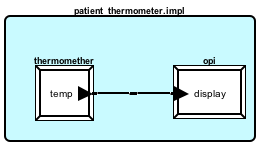
\includegraphics[height=1.5in]{figures/patient_thermometer.png}
    	\caption{AADL model of simple thermometer}
    \end{center}
    \label{figure:patient_thermometer}
\end{figure}

\singlespacing
\begin{lstlisting}[language=aadl, frame=single, gobble=0, caption={AADL model of simple thermometer}, label={listing:patient_thermometer}]
	package Thermometer
	public
	with Base_Types;
		system patient_thermometer
		end patient_thermometer;

		system implementation patient_thermometer.impl
		subcomponents
			thermomether : device thermometer_device.impl;
			opi : device operator_interface.impl;
		connections
			tdn : port thermomether.temp -> opi.display;
		end patient_thermometer.impl;

		device operator_interface
		features
			display : in data port Base_Types::Integer;
		end operator_interface;

		device implementation operator_interface.impl
		end operator_interface.impl;

		device thermometer_device
		features
			temp : out data port Base_Types::Integer;
		end thermometer_device;

		device implementation thermometer_device.impl
		end thermometer_device.impl;
	end Thermometer;
\end{lstlisting} 
\doublespacing
%another example: https://wiki.sei.cmu.edu/aadl/images/7/73/AADLV2Overview-AADLUserDay-Feb_2010.pdf (slide 16)

Recently AADL becomes a new market standard. There are lots of tools for AADL models analysis, such as: STOOD \footnote{http://www.ellidiss.com/products/stood}, ADELE \footnote{https://wiki.sei.cmu.edu/aadl/index.php/Adele}, Cheddar \footnote{http://beru.univ-brest.fr/~singhoff/cheddar}, AADLInspector \footnote{http://www.ellidiss.com/products/aadl-inspector} or Ocarina \footnote{http://www.openaadl.org}.

What is important, AADL is for architectural description. It should not be compared with UML suites, which allows to link with source code.


\subsection{OSATE}
\label{background:aadl:osate}
Open Source AADL Tool Environment (OSATE) is a set of plug-ins on top of the open-source Eclipse platform. It provides a toolset for front-end processing of AADL models. OSATE is developed mainly by SEI (Software Engineering Institute - CMU) \footnote{http://www.aadl.info/aadl/currentsite/tool/osate.html}. Latest available version of OSATE in the time when this work was published is OSATE2 \footnote{https://wiki.sei.cmu.edu/aadl/index.php/Osate\_2}.



\section{BLESS}
\label{background:bless}
BLESS (Behavior Language for Embedded Systems with Software) is AADL annex sublanguage defining behavior of components. The goal of BLESS is automatically-checked correctness proofs of AADL models of embedded electronic systems with software.

BLESS contains three AADL annex sublanguages:
\begin{itemize} \itemsep1pt \parskip0pt \parsep0pt
	\item Assertion - it can be attached individually to AADL features (e.g. ports)
	\item subBLESS - can be attached only to subprograms; it has only value transformations and Assertions without time expressions
	\item BLESS - it can be attached to AADL thread, device or system components; it contains states, transitions, timeouts, actions, events and Assertions with time expressions...
\end{itemize}

How it fits into the picture. Why it was developed. Corectness prove in AADL + behavior \cite{Bless:Paper}, from which we can generate SPARK Ada code.



\section{SPARK Ada}
\label{background:spark}

%http://www.cs.swan.ac.uk/~csetzer/lectures/critsys/09/critsysfinal2.pdf

First version of Ada programming language - Ada 83 - was designed to meet the US Department of Defence Requirements formalized in "Steelman" document \footnote{http://www.adahome.com/History/Steelman/steelman.htm}. Since that time, Ada evolved. There were Ada 95, Ada 2005 and Ada 2012 (released in December 10, 2012) \footnote{http://www.ada2012.org}. Ada is actively used in many Real-World projects\footnote{http://www.seas.gwu.edu/~mfeldman/ada-project-summary.html}, e.g. Aviation (Boeing \footnote{http://archive.adaic.com/projects/atwork/boeing.html}), Railway Transportation, Commercial Rockets, Satellites and even Banking. One of the main goals of Ada is to ensure software correctness and safety.

\begin{figure}[ht]%t=top, b=bottom, h=here
    \begin{center}
    	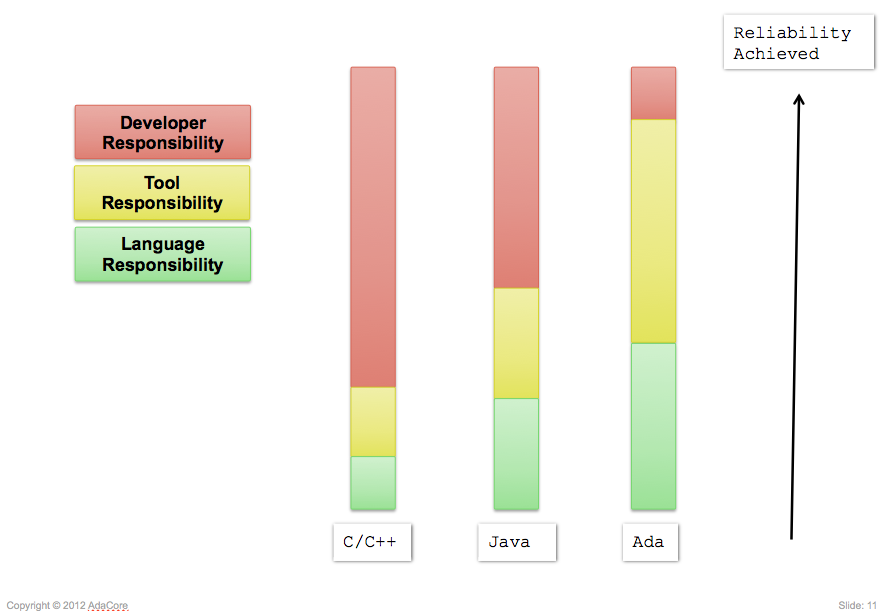
\includegraphics[height=3.5in]{figures/developer_responsibility_in_ada.png}
    	\caption{Developer responsibility in Ada\protect\footnotemark. }    	
    \end{center}
\end{figure}
\footnotetext{http://www.slideshare.net/AdaCore/ada-2012}

SPARK is a programming language and static verification technology designed specifically for the development of high integrity software. It is a "safe" subset of Ada designed to be susceptible to formal methods, accompanied with a set of approaches and tools. Using SPARK, a developer takes a Z specification and performs a stepwise refinement from the specification to SPARK code. For each refinement step a tool is used to produce verification conditions (VC's), which are mathematical theorems. If the VC's can be proved then the refinement step will be known to be valid. However if the VC's cannot be proved then the refinement step may be erroneous \footnote{http://www.dwheeler.com/lovelace/s17s4.htm}.

% Barnes' 15.7 where SPARK is used

First version was designed over 20 years ago. SPARK has established a track record of use in embedded and critical systems across a diverse range of industrial domains where safety and security are paramount \cite{Barnes:Book}. 

SPARK provides a significant degree of automation in proving exception freedom \cite{Spark:Article}. SPARK excludes some Ada constructs to make static analysis feasible \cite{Spark:Article}. Additionally SPARK contains tool-set for Software Verification:
\begin{itemize} \itemsep1pt \parskip0pt \parsep0pt
	\item Examiner - analyze code and ensures that it conforms to the SPARK language; also verify program to some extent using Verification Conditions (VC)
	\item Simplifier - simplify Verification Conditions generated by Examiner
	\item Proof Checker - prove the Verification Conditions
\end{itemize}

First version of SPARK was based on Ada 83. The second version (SPARK 95) - on Ada 95. SPARK 2005 is based on Ada 2005. It is a subset of Ada 2005 with annotations. The annotation language support flow analysis and formal verification. Annotations are encoded in Ada comments (via the prefix \lstinline{--#}). It makes every SPARK 2005 program, valid Ada 2005 program. Figure \ref{listing:Odometer2005} shows example SPARK 2005 package specification.

\singlespacing
\begin{lstlisting}[language=ada, frame=single, gobble=0, caption={SPARK 2005 code: Odometer \cite{Barnes:Book}}, label={listing:Odometer2005}]
	package Odometer
	--# own Trip, Total : Integer;
	is
		procedure Zero_Trip;
		--# global out Trip;
		--# derives Trip from ;
		--# post Trip = 0;

		function Read_Trip return Integer;
		--# global in Trip;

		function Read_Total return Integer;
		--# global in Total;

		procedure Inc;
		--# global in out Trip, Total;
		--# derives Trip from Trip & Total from Total;
		--# post Trip = Trip~ + 1 and Total = Total~ + 1;

	end Odometer;
\end{lstlisting} 
\doublespacing

SPARK 2005 does not include constructs such as pointers, dynamic memory allocation or recursion \cite{Spark:Article}.

SPARK 2014 \footnote{http://www.spark-2014.org} is based on Ada 2012 programming language targeted at safety- and security-critical applications \cite{Spark2014:Paper}. Since Ada 2012 contains contracts, there is no need to use annotations like in SPARK 2005. Thus SPARK 2014 is subset of Ada 2012. It contains all features of Ada 2012 except:
\begin{itemize} \itemsep1pt \parskip0pt \parsep0pt
 	\item Access types (pointers)
 	\item Exceptions
	\item Aliasing between variables
	\item Concurrency features of Ada (Tasking) - it's part of SPARK 2014 road-map to include support for tasking in the future, although likely not this year
	\item Side effects in expressions and functions
\end{itemize}

Sample mapping from SPARK 2005 to 2014 is shown on table \ref{table:spark2005and2014mapping}. Complete mapping can be found in SPARK 2014 documentation \footnote{http://docs.adacore.com/spark2014-docs/html/lrm/mapping-spec.html} \cite{Spark2014refManual:Online}.

\singlespacing
\begin{table}[!ht]
	\caption{Sample SPARK 2005 to 2014 mapping.}
	\label{table:spark2005and2014mapping}
	\centering
  	\begin{tabular}{ | p{3in} | p{3in} |}
	  	%\multicolumn{1}{c}{\textbf{AADL/BLESS}} & \textbf{SPARK Ada}\\

		\hline
		\multicolumn{1}{|c|}{\textbf{SPARK 2005}} & \multicolumn{1}{|c|}{\textbf{SPARK 2014}} \\ \hline

		\begin{lstlisting}
			--# global in out X, Y;
		\end{lstlisting} 
		& 
		\begin{lstlisting}[language=ada2012]
			with Global  => (In_Out => (X, Y));
		\end{lstlisting} 

		\\ \hline

		\begin{lstlisting}
			--# derives X from Y &
			--#         Y from X;
		\end{lstlisting} 
		& 
		\begin{lstlisting}[language=ada2012]
			Depends => (X => Y,
			            Y => X);
		\end{lstlisting}

		\\ \hline

		\begin{lstlisting}
			--# pre Y /= 0 and
			--#     X > Integer'First;
		\end{lstlisting} 
		& 
		\begin{lstlisting}[language=ada2012]
			with Pre  => Y /= 0 and 
			             X > Integer'First;
		\end{lstlisting}

		\\ \hline

		\begin{lstlisting}
			--# post X = Y~ and Y = X~;
		\end{lstlisting} 
		& 
		\begin{lstlisting}[language=ada2012]
			with Post => (X = Y'Old and Y = X'Old);
		\end{lstlisting} 

		\\ \hline
	\end{tabular}
\end{table}
\doublespacing

SPARK 2014 does not contains Examiner. Instead, proofs are made by gnatPROVE.
The notion of executable contracts in Ada 2012, was inspired by SPARK. The previous Odometer example in SPARK 2014 is shown in figure \ref{listing:Odometer2014}.

\singlespacing
\begin{lstlisting}[language=ada2012, frame=single, gobble=0, caption={SPARK 2014 code: Odometer}, label={listing:Odometer2014}]
	package Odometer
	with SPARK_Mode
	Abstract_State => (Trip, Total)
	is
		procedure Zero_Trip
		with Global => (Output => (Trip)),
		   Depends => (Trip => null),
		   Post => (Trip = 0);

		function Read_Trip return Integer
		with Global => (Input => (Trip));

		function Read_Total return Integer
		with Global => (Input => (Total));

		procedure Inc	   
		with Global => (In_Out => (Trip, Total)),
			Depends => (Trip => Trip, Total => Total),
			Post => Trip = Trip'Old + 1 and Total = Total'Old + 1;

	end Odometer;
\end{lstlisting} 
\doublespacing

Fundamental SPARK contracts:

\singlespacing
\begin{center}
	\begin{longtable}{| p{1.5in} | p{1.5in} | p{3in} |}
		\caption{Fundamental SPARK annotations}
		\label{table:SparkAnnotations}
		\\
		\hline
		\multicolumn{1}{|c|}{\textbf{SPARK 2005}} & \multicolumn{1}{|c|}{\textbf{SPARK 2014}} & \multicolumn{1}{|c|}{\textbf{Description}} \\ \hline
		\endfirsthead

		\multicolumn{3}{c}%
		{{\bfseries \tablename\ \thetable{} -- continued from previous page}} \\
		\hline 
		\multicolumn{1}{|c|}{\textbf{SPARK 2005}} & \multicolumn{1}{|c|}{\textbf{SPARK 2014}} & \multicolumn{1}{|c|}{\textbf{Description}} \\ \hline
		\endhead

		\hline \multicolumn{3}{|r|}{{Continued on next page}} \\ \hline
		\endfoot

		\hline %\hline
		\endlastfoot

		\begin{lstlisting}
			--# global
		\end{lstlisting} 
		& 
		\begin{lstlisting}[language=ada2012]
			Global
		\end{lstlisting} 
		& 
		list of used global variables within subprogram 

		\\ \hline

		\begin{lstlisting}
			--# derives
		\end{lstlisting} 
		& 
		\begin{lstlisting}[language=ada2012]
			Depends
		\end{lstlisting} 
		& 
		describe dependencies between variables

		\\ \hline

		\begin{lstlisting}
			--# own 
		\end{lstlisting} 
		& 
		\begin{lstlisting}[language=ada2012]
			Abstract_State
		\end{lstlisting} 
		& 
		declare variables defined in package body

		\\ \hline

		\begin{lstlisting}
			--# initializes
		\end{lstlisting} 
		& 
		\begin{lstlisting}[language=ada2012]
			initializes
		\end{lstlisting} 
		& 
		indicates variables, which are initialized

		\\ \hline

		\begin{lstlisting}
			--# inherit
		\end{lstlisting} 
		& 
		not needed
		& 
		allows to access entities of other packages

		\\ \hline

		\begin{lstlisting}
			--# pre
		\end{lstlisting} 
		& 
		\begin{lstlisting}[language=ada2012]
			Pre
		\end{lstlisting} 
		& 
		pre condition

		\\ \hline
		

		\begin{lstlisting}
			--# post
		\end{lstlisting} 
		& 
		\begin{lstlisting}[language=ada2012]
			Post
		\end{lstlisting} 
		& 
		post condition

		\\ \hline
		

		\begin{lstlisting}
			--# assert
		\end{lstlisting} 
		& 
		\begin{lstlisting}[language=ada2012]
			Assert
		\end{lstlisting} 
		& 
		assertion

		\\ \hline
	\end{longtable}
\end{center}
\doublespacing

It is possible to mix SPARK 2014 with Ada 2012. However, only the part which is SPARK 2014 compliant will be verified. Usually SPARK is used in the most critical parts of Software Systems \cite{Spark:IndustrialExp}. It means, that some part is written in e.g. Ada or C++ and the rest in SPARK. The reason of that is the SPARK limitation and lack of necessity to verify some modules.
% http://docs.adacore.com/spark2014-docs/html/ug/spark_2014.html#mixing-spark-code-and-ada-code

The most popular IDE for SPARK Ada is GNAT Programming Studio \footnote{http://libre.adacore.com/tools/gps}.

There is also plugin for Eclipse: GNATbench \footnote{https://www.adacore.com/gnatpro/toolsuite/gnatbench/} created by AdaCore. 
Tools for correctness proving.


\subsection{GNAT compiler and Programming Studio}
\label{background:spark:gps}
GNAT compiler is front end of gcc...
IDE for SPARK Ada programs development. Includes proving tools. E.g. Sireum Bakar (developed by SAnToS lab) or GNATprove.


\subsection{Ravenscar Tasking Subset}
\label{background:spark:ravenscar}

RavenSPARK is subset of the SPARK Ravenscar Profile (which is subset of Ada tasking). The Ravenscar Profile provides a subset of the tasking facilities of Ada95 and Ada 2005 suitable for the construction of high-integrity concurrent programs \cite{Ravenscar:Online}.

The Ravenscar Profile is a subset of the tasking model, restricted to meet the real-time community requirements for determinism, schedulability analysis and memory-boundedness, as well as being suitable for mapping to a small and efficient run-time system that supports task synchronization and communication, and which could be certifiable to the highest integrity levels. The concurrency model promoted by the Ravenscar Profile is consistent with the use of tools that allow the static properties of programs to be verified. Potential verification techniques include information flow analysis, schedulability analysis, execution-order analysis and model checking. These techniques allow analysis of a system to be performed throughout its development life cycle, thus avoiding the common problem of finding only during system integration and testing that the design fails to meet its non-functional requirements. \cite{Ravenscar:Article}

Concurrent programs require the use of different specification and verification techniques from sequential programs. For this reason, tasks, protected units and objects, and synchronization features are currently excluded from SPARK 2014 \footnote{http://docs.adacore.com/spark2014-docs/html/lrm/tasks-and-synchronization.html} \cite{Spark2014refManual:Online}.

To create a task, the task type has to be declared and task variable of this type. Ravenscar does not allow dynamic task creation. Thus, all tasks have to exists for the full lifetime of the program. \cite{IssuesWithRavenscar:Paper} Tasks can be declared only in packages. Not in subprograms or in other tasks. \cite{Barnes:Book} The priority of each tasks has to be specified by \lstinline{pragma Priority}. [what is priorities range?] Listing \ref{lst:SampleTask} shows sample package with two tasks.

\singlespacing
\begin{lstlisting}[frame=single, gobble=0, caption={Sample tasks}, label={lst:SampleTask}]
	package Some_Pkg
	--# own task t1 : Task1;
	--#     task t2 : Task2;
	is
		task type Task1
		is
			pragma Priority(10);
		end Task1;

		task type Task2
		is
			pragma Priority(9);
		end Task2;

	end Some_Pkg;
\end{lstlisting} 
\doublespacing

Declared tasks have to be implemented in the package body (listing \ref{lst:SampleTaskBody}).

\singlespacing
\begin{lstlisting}[frame=single, gobble=0, caption={Sample tasks body}, label={lst:SampleTaskBody}]
	package body Some_Pkg
	is
		t1 : Task1;
		t2 : Task2;

		task body Task1
		is
		begin
			loop
				-- implementation;
			end loop;
		end Task1;

		task body Task2
		is
		begin
			loop
				-- implementation;
			end loop;
		end Task2;

	end Some_Pkg;
\end{lstlisting} 
\doublespacing

There are two ways to access variable in different tasks:
\begin{itemize}
    \item It has to be protected object
    \item It has to be atomic type
\end{itemize}


Protected object encapsulate variable, in such a way that it is accessible, only through protected subprograms. This mechanism use locking, to ensure atomicity. Protected type declaration is similar to task: specification and body has to be defined. Listing \ref{lst:SampleTasksWithProtectedType} shows sample tasks with protected type \lstinline{Integer_Store}, which enable to share Integer variable between tasks. What is important, protected type has to be declared before tasks, which will use it. Otherwise, it will not be visible for them.

\singlespacing
\begin{lstlisting}[frame=single, gobble=0, caption={Sample tasks with protected object}, label={lst:SampleTasksWithProtectedType}]
	package Some_Pkg
	--# own protected Shared_Var : Integer_Store (Priority => 11);
	--#     task t1 : Task1;
	--#     task t2 : Task2;
	is
	    protected type Integer_Store
	    is
	        pragma Priority (11);

	        function Get return Integer;
	        --# global in Integer_Store;

	        procedure Put(X : in Integer);
	        --# global out Integer_Store;
	        --# derives Integer_Store from X;
	    private
	        TheStoredData : Integer := 0;
	    end Integer_Store;

	    task type Task1
	      --# global out Shared_Var;
	    is
	        pragma Priority(10);
	    end Task1;

	    task type Task2
	      --# global in Shared_Var;
	    is
	        pragma Priority(9);
	    end Task2;

	end Some_Pkg;
\end{lstlisting}
\doublespacing

Protected type body also has to be defined in package body (listing \ref{lst:SampleTasksWithProtectedTypeBody}).

\singlespacing
\begin{lstlisting}[frame=single, gobble=0, caption={Sample tasks with protected object body}, label={lst:SampleTasksWithProtectedTypeBody}]
	package body Some_Pkg
	is
	    Shared_Var : Integer_Store;
	    t1 : Task1;
	    t2 : Task2;

	    protected body Integer_Store is
	        function Get return Integer
	        --# global in TheStoredData;
	        is
	        begin
	            return TheStoredData;
	        end Get;

	        procedure Put(X : in Integer)
	        --# global out TheStoredData;
	        --# derives TheStoredData from X;
	        is
	        begin
	            TheStoredData := X;
	        end Put;
	    end Integer_Store;

	    task body Task1
	    is
	    begin
	        loop
	            Shared_Var.Put(5);
	        end loop;
	    end Task1;

	    task body Task2
	    is
	        Local_Var : Integer;
	    begin
	        loop
	            Local_Var := Shared_Var.Get;
	        end loop;
	    end Task2;

	end Some_Pkg;
\end{lstlisting} 
\doublespacing

\lstinline{Task1} is writing to \lstinline{Shared_Var} and \lstinline{Task2} is reading \lstinline{Shared_Var}. The highest priority is assigned to protected object, to ensure atomicity during operations on it. The lowest priority is assigned to \lstinline{Task2}, which is reading \lstinline{Shared_Var}. Reading is usually less expensive operation than writing. Thus, to avoid starvation, \lstinline{Task1} has higher priority than \lstinline{Task2}. Notice, that \lstinline{Shared_Var} is declared in package body, but refined in package specification.

Protected variables may not be used in proof contexts. Thus, if we try to use protected variable in proofs (pre- or postcondition), then SPARK Examiner returns \lstinline{Semantic Error 940 - Variable is a protected own variable. Protected variables may not be used in proof contexts.}. Formal reasoning about interactions and especially temporal properties require other techniques such as model checking and lie outside the scope of SPARK \cite{Barnes:Book}. To preserve opportunity to use pre- and postconditions, atomic types have to be used.

To declare atomic type, we have to use \lstinline{pragma Atomic}. However, there is restriction, that \lstinline{pragma Atomic} cannot be applied to predefined type such as Integer. Thus, we have to define our custom type (which can be just rename of Integer) and apply \lstinline{pragma Atomic} on this type. Listing \ref{lst:SampleTasksWithAtomicType} presents previous example with atomic types instead of protected objects.

\singlespacing
\begin{lstlisting}[frame=single, gobble=0, caption={Sample tasks with atomic type}, label={lst:SampleTasksWithAtomicType}]
	package Some_Pkg
	--# own Shared_Var;
	--#     task t1 : Task1;
	--#     task t2 : Task2;
	--# initializes Shared_Var;
	is
	    type Int32 is new Integer;
	    
	    task type Task1
	      --# global out Shared_Var;
	    is
	        pragma Priority(10);
	    end Task1;

	    task type Task2
	      --# global in Shared_Var;
	    is
	        pragma Priority(9);
	    end Task2;

	end Some_Pkg;

	package body Some_Pkg
	is    
	    Shared_Var : Int32 := 0;
	    t1 : Task1;
	    t2 : Task2;

	    task body Task1
	    is
	    begin
	        loop
	            Shared_Var := 5;
	        end loop;
	    end Task1;

	    task body Task2
	    is
	        Local_Var : Integer;
	    begin
	        loop
	            Local_Var := Integer(Shared_Var);
	        end loop;
	    end Task2;

	end Some_Pkg;
\end{lstlisting}
\doublespacing

Be aware that \lstinline{pragma atomic} does not guaranty atomicity. In most cases, atomic types should not be used for tasking. Instead, protected types should be used.
% precise! http://en.wikibooks.org/wiki/Ada_Programming/Pragmas/Atomic

Another important thing in tasking is Time library: \lstinline{Ada.Real_Time}. It allows to run task periodically, using \lstinline{delay until} statement, which suspends task until specified time. To use \lstinline{delay} in the task, it has to be declared in \lstinline{declare} annotation: \lstinline{--# declare delay;} \cite{Barnes:Book}.

Details about tasking in SPARK are well described in Chapter 8 of Barnes' book \cite{Barnes:Book}. The "Guide for the use of the Ada Ravenscar profile in high integrity systems" \cite{Ravenscar:Article} and the official Ravenscar Profile documentation (which includes examples) \cite{Ravenscar:Online} might be useful as well. The limitations of Tasking in SPARK are reviewed in Audsley's and Welllings' paper \cite{IssuesWithRavenscar:Paper}.


\section{SPARK Ada Verification}
\label{background:sparkverification}

%http://docs.adacore.com/sparkdocs-docs/

Verification - what is that
verification vs validation

SPARK tools
FDL is the modelling language of the SPARK proof tools. 

\begin{figure}[ht]%t=top, b=bottom, h=here
    \begin{center}
    	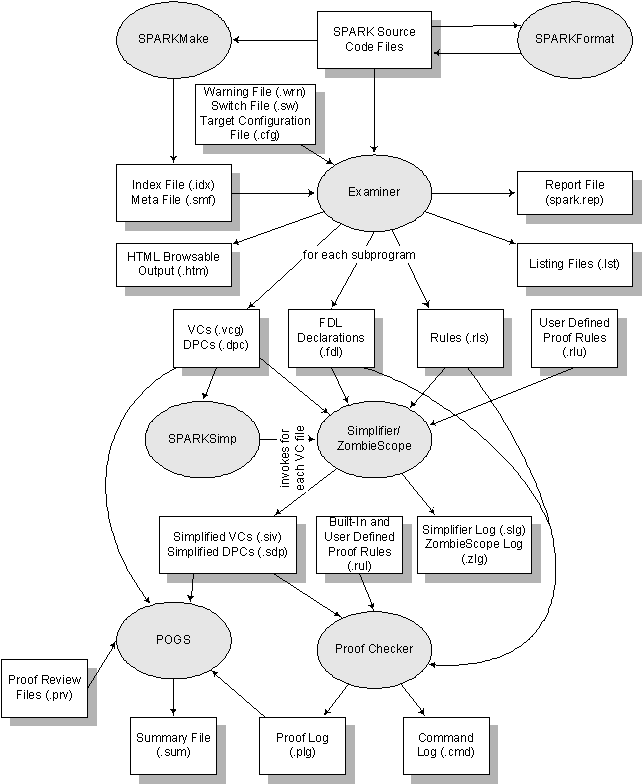
\includegraphics[height=7in]{figures/spark-tools.png}
    	\caption{Relationship of the Examiner and Proof Tools\protect\footnotemark.}
    \end{center}
\end{figure}
\footnotetext{http://docs.adacore.com/sparkdocs\-docs/Examiner\_UM.htm}



\subsection{SPARK Examiner}
\label{verification:examiner}

The main SPARK verification tool is Examiner. It supports several levels of analysis:
\begin{itemize}
	\item checking of SPARK language syntactic and static semantic rules
	\item data flow analysis
	\item data and information flow analysis
	\item formal program verification via generation of verification conditions
	\item proof of absence of run-time errors
	\item dead path analysis
\end{itemize}

There is also an option to make the Examiner perform syntax checks only. Using this option on a source file does not require access to any other units on which the file depends, so files can be syntax checked on an individual basis. This allows any syntax errors to be corrected before the file is included in a complex examination.  This option must only be used as a pre-processor: the absence of syntax errors does NOT indicate that the source text is a legal SPARK program. \cite{Examiner:Online} (THIS PART IS COPY AND PASTE FROM Examiner doc - is it ok?)

Put here some examples: method without contract, examine, add specification, pass Examiner.

During implementation, code was regularly checked using SPARK Examiner.

What is very important, Examiner can perform data and information analysis of Ravenscar programs in exactly the same manner as for sequential programs \cite{Ravenscar:Online}. Unfortunately it does not allow protected objects in proof annotations (pre- and post-conditions).

When some parts of the system are written in full Ada (with non-valid SPARK constructs), then Examiner returns error. Ada parts can be excluded from Examiner analysis using \lstinline{--# hide} annotation. The, only warning \lstinline{10 - The body of subprogram Main is hidden - hidden text is ignored by the Examiner.} is returned by Examiner.

Examiner use SPARK index file to locate files necessary for verification. \cite{Barnes:Book}

Examiner can be used with \lstinline{spark} command and appropriate flags described in Examiner Manual \cite{Examiner:Online}.

%http://docs.adacore.com/sparkdocs-docs/SPARK_GPS.htm
%[screenshot - take from 721 paper]
To use Examiner in GNAT Programming Studio:
\begin{itemize}
	\item Run SPARK Make (right click on project / SPARK / SPARK Make)
	\item Set SPARK index file (to spark.idx generated by SPARKMake) [add photo from 721 paper]
	\item (optionally) set configuration file (Standard.ads)
	\item Choose appropriate version of SPARK (95 or 2005)
	\item Choose mode: Sequential (for single tasking programs) or Ravenscar (for multitasking programs)
\end{itemize}

To generate verification conditions (VCs), the \lstinline{-vcg} switch has to be used. It can be set in GNAT Programming Studio (Project / Edit project properties / Switches / Examiner / Generate VCs).
In addition to verification conditions, Examiner can check dead path conjectures. It checks, whether all of the program is useful. To generate dead path conjectures, the \lstinline{-dpc} switch has to be used. It can be also set in GNAT Programming Studio (Project / Edit project properties / Switches / Examiner / Generate DPCs).


\subsubsection{Flow analysis}
\label{verification:examiner:flowanalysis}
%http://www.cs.swan.ac.uk/~csetzer/lectures/critsys/09/critsysfinal2.pdf
There are two types of flow analysis:
\begin{itemize}
	\item Data flow analysis:
	\begin{itemize}
		\item Checks input/output behavior of parameters and variables.
		\item Checks initialization of variables.
		\item Checks that changed and imported variables are used later (possibly as output variables).
	\end{itemize}
	\item Information flow analysis - verifies interdependencies between variables.
\end{itemize}

In data flow analysis, Examiner checks if input parameters are not modified, but used at least once (in at least one branch of program). In the same factor, output parameters cannot be read (before initialization) and has to be initialized (in all branches of program). Input/output parameters has to be both read and write (changed). In similar way, Examiner verify the global variables (specified in annotations). Functions can use only input parameters and can only read global variables. Therefore functions do not have side effects. 

Global variables defined in package body (thus private) has to be declared by \lstinline{--# own} annotation in package specification. If variable is also initialized, \lstinline{--# initializes} annotation has to be used. In Ada, to use package in another package, \lstinline{with} clause has to be used. In SPARK Ada, additionally \lstinline{--# inherits} annotation has to be specified.

In information flow analysis, dependencies between variables are analyzed. These dependencies are specified by \lstinline{--# derives} annotation.


\subsubsection{Verification conditions}
\label{verification:examiner:vc}

To generate verification conditions, two kinds of annotations are relevant for Examiner:
\begin{itemize}
	\item pre-conditions: \lstinline{--# pre}
	\item post-conditions: \lstinline{--# post}
\end{itemize}

Notion of pre- and post-conditions represents Hoare logic. More precisely, Hoare triple: 

\begin{equation} \label{eq:hoare_triple}
	\{P\} C \{Q\}
\end{equation}

P and Q are assertions. C is a command (action) performed between them. P is pre-condition and Q is post-condition.

Additionally, assertions (\lstinline{--# assert}) and checks (\lstinline{--# check}) can be specified in procedure body. Then additional verification conditions are generated.

Functions does not have side effects (as stated in \ref{verification:examiner:flowanalysis}), thus only pre-condition can be applied. However, there is annotation \lstinline{--# return}, which specify function return value.

Verification conditions are generated depended on number of paths in subprogram. Analysis are perform backwards, in other words: we start from post-conditions and consider what must holds before. Flow analysis is well described in chapter 11 of Barnes' book \cite{Barnes:Book}.



\subsection{SPARK Simplifier}
\label{verification:simplifier}

Simplifier can discharge (prove correctness) of verification conditions (VCs) generated by Examiner, but not proved by Examiner. \cite{Simplifier:Online} 



\subsection{ZombieScope}
\label{verification:zombiescope}

ZombieScope is a SPARK tool, that analyses SPARK code to find dead paths, i.e. paths through the code that can never be executed.


\subsection{Victor}
\label{verification:victor}

Victor is a tool to translate SPARK verification conditions (VCs), as generated by the Examiner, into SMT-LIB (file format used to communicate with SMT solvers). \cite{Victor:Online} SMT (Satisfiability Modulo Theories) solver is a tool...
experimental feature
Integrated with SPARKSimp (by -victor flag) and POGS.


\subsection{Proof Checker}
\label{verification:proofchecker}

% Barnes' book: 12.12
Only mention. It is hardcore.

\subsection{SPARKSimp Utility}
\label{verification:sparksimp}
SPARKSimp is a simple "make" style tool for the SPARK analysis tools. Currently, it supports the Simplifier, ZombieScope and ViCToR. It applies the Simplifier (and ViCToR, if requested, please see the Victor\_Wrapper user manual \cite{Victor:Online} for more information) to all .vcg files and ZombieScope to all .dpc files it finds in a directory tree. \cite{SPARKSimp:Online} 



\subsection{Proof Obligation Summarizer (POGS)}
\label{verification:pogs}

The Proof ObliGation Summarizer tool (POGS) reads and understands the structure of the verification condition files. It reports the status of proofs and dead path analyses in a human-readable form. \cite{POGS:Online}

\subsection{AUnit}
\label{background:spark:aunit}
AUnit is Unit Test Framework for Ada language. It can be also applied for verify SPARK Ada programs.
AUnit tutorials \cite{AUnitTutorials:Online}
AUnit Cookbook \cite{AUnitCookbook:Online}


\subsection{Sireum Bakar}
\label{background:spark:sireum}
Overview: symbolic execution, Pilar, Kiasan and Alir \cite{Hari:Thesis}.
Sireum Kiasan \cite{Kiasan:Paper} is a tool, which use symbolic execution for finding possible paths in program.
Plugin for GNAT Programming Studio (SPARK 2005 and 2014 under development).
Plugin for Eclipse (only for SPARK 2005).
No support for Ravenscar profile.
Separated sequential parts can be verified (Odometer?). Sequential version of \lstinline{Max_Drug_Per_Hour_Watcher}?


\subsection{GNAT Prove}
\label{background:spark:gnatprove}
GNATprove \footnote{http://www.open-do.org/projects/hi-lite/gnatprove/} is a formal verification tool for SPARK 2014 programs. It interprets SPARK Ada annotations exactly like they are interpreted at run time during tests.
% http://docs.adacore.com/spark2014-docs/html/ug/gnatprove.html
% only for SPARK 2014


\section{AADL/BLESS to SPARK Ada code generation}
\label{background:codegen}
The ultimate goal of long term research, this thesis is part of, is AADL (with BLESS) to SPARK Ada translation.


\subsection{Ocarina}
\label{background:codegen:ocarina}
Ocarina \cite{Ocarina:Paper,Ocarina:Paper} generates code from an AADL architecture model to an Ada application running on top of PolyORB framework. In this context, PolyORB acts as both the distribution middleware and execution runtime on all targets supported by PolyORB.
It generate Ada 2005 and C code.
Since mid-2009, Telecom ParisTech is no longer involved in Ocarina, and is developing another AADL tool-chain, based on Eclipse, codenamed RAMSES \cite{Ocarina:About:Online}.

examples on github

run:
ocarina -x scenario.aadl



\subsection{Ramses}
\label{background:codegen:ramses}
% very shortly
RAMSES is a model transformation framework dedicated to the refinement of AADL models. It contains code generation plug-in.
% http://www.aadl.info/aadl/downloads/committee/feb2013/presentations/RAMSES_status_2013_06_02_format.pdf
% https://wiki.sei.cmu.edu/aadl/index.php/OSATE_2_on_the_command-line
%!TEX root = etdrtemplate.tex
% +--------------------------------------------------------------------+
% | Sample Chapter 3
% +--------------------------------------------------------------------+

\cleardoublepage

% +--------------------------------------------------------------------+
% | Replace "This is Chapter 3" below with the title of your chapter.
% | LaTeX will automatically number the chapters.
% +--------------------------------------------------------------------+

\chapter{PCA Pump Prototype}
\label{pcapump}

Overview of PCA Pump and issues, which MDCF/ICE will solve.
In this thesis, only the operation module is implemented.


\section{PCA Pump Requirements Document}
\label{pcapump:requirements-doc}
Selected use cases for implementation?
Overview of issues solved: 
* Bolus options: FBasal + FPatient or FPatient


\section{PCA Pump AADL/BLESS Models}
\label{pcapump:aadl-bless-models}
Selected modules for implementation. Pictures etc.


\section{BeagleBoard-XM}
\label{pcapump:beagleboard}
First step was create PCA Pump prototype on BeagleBoard-xM.

BeagleBoard-xM is Embedded device with AM37x 1GHz ARM processor (Cortex-A8 compatible). It has 512 MB RAM, 4 USB 2.0 ports, HDMI port, 28 General-purpose input/output (GPIO) ports and Linux Operating System (on microSD card). All these properties makes this device good candidate for prototyping PCA Pump.

Expansion port 14 and 28
GPIO158
Java Program to Run the pump for 10 seconds

There is no existing SPARK/Ada compiler running on ARM system. Hence, to compile SPARK/Ada program for ARM device, we need to perform cross-compilation on other machine. There is GNAT compiler \cite{Horn:Thesis} created by AdaCore, but there was no cross-compiler for ARM. However AdaCore was working on it. They had working version in 2013, but tested only on their target, Android-based device. BeagleBoard-xM is coming with Linux Angstrom Operating System. There is possibility to install Android on BeagleBoard-xM, but still not warranty everything will be working. Cooperation with AdaCore allowed to cross-compile SPARK/Ada program for BeagleBoard-xM.

Include source of simple program?
GNAT cross-compiler only for Linux Platform (cross-compilation has to be done on Linux).


\section{PCA Pump Prototype Implementation}
\label{pcapump:implementation}

Currently SPARK 2014 does not support tasking \cite{Spark2014refManual:Online}. For SPARK 2005, GNAT compiler provides Ravenscar Profile \cite{Ravenscar:Online}. It provides a subset of the tasking facilities of Ada95 and Ada 2005 suitable for the construction of high-integrity concurrent programs.

Issues: Ravenscar Profile, how to deal with different boluses (look at UMinn requirements and annotations for our doc).
Look at annotated PCA Pump Req document.

\subsection{Concurrency in SPARK}
\label{pcapump:implementation:concurrency}

Concurrent programs require the use of different specification and verification techniques from sequential programs. For this reason, tasks, protected units and objects, and synchronization features are currently excluded from SPARK 2014 \footnote{http://docs.adacore.com/spark2014-docs/html/lrm/tasks-and-synchronization.html} \cite{Spark2014refManual:Online}.

In SPARK 2005, concurrency is enable using the Ravenscar profile \cite{Ravenscar:Online}. 

\cite{Ravenscar:Article}

\subsection{Interface for Integrated Clinical Environment}
\label{pcapump:implementation:ice}

Describe communication with MDCF/ICE. PCA Pump ports for that etc.
%!TEX root = etdrtemplate.tex
% +--------------------------------------------------------------------+
% | Sample Chapter 4
% +--------------------------------------------------------------------+

\cleardoublepage

% +--------------------------------------------------------------------+
% | Replace "This is Chapter 4" below with the title of your chapter.
% | LaTeX will automatically number the chapters.
% +--------------------------------------------------------------------+

\chapter{AADL/BLESS to SPARK/Ada translation}
\label{codegen}

First step was to create mock (based on doc, aadl models and implemented PCA Pump).
Prototyping Embedded Systems using AADL lasts for a few years \cite{PrototypyingAadl:Paper}.

\section{AADL/BLESS to SPARK/Ada mapping}
\label{codegen:mapping}

%https://wiki.sei.cmu.edu/aadl/images/4/40/13_04_24-AADL-Code_Generation.pdf

%https://wiki.sei.cmu.edu/aadl/images/7/73/AADLV2Overview-AADLUserDay-Feb_2010.pdf (slide 35: port connections)

Mapping is driven by "Architecture analysis \& Design Language (AADL) V2 Programming Language Annex Document" \cite{AnnexDoc13}. Ocarina tool suite (based on older AADL annex documents \cite{Ocarina:Article}) was also helpful in understanding of AADL to Ada translation.
Only high level mapping is done. No implementation (thread interactions) like Ocarina does. 

3 areas of mapping:
* data types
* thread -> subprograms
* subprogram -> subprogram

\subsection{Data types mapping}
\label{codegen:mapping:data}

\subsection{AADL ports mapping}
\label{codegen:mapping:ports}

Proposed ports mapping shown in table \ref{table:aadl2spark_ports} is based on AADL runtime services from Annex 2 to "Programming Language Annex Document" \cite{AnnexDoc13}.

% maybe split right column into 2 rows: spec and body?
\begin{center}
	\begin{longtable}{| p{2in} | p{4in} |}
	
		\caption{AADL to SPARK ports mapping.}
		\label{table:aadl2spark_ports}
		\\
		\hline
		\multicolumn{1}{|c|}{\textbf{AADL/BLESS}} & \multicolumn{1}{|c|}{\textbf{SPARK/Ada}} \\ \hline
		\endfirsthead

		\multicolumn{2}{c}%
		{{\bfseries \tablename\ \thetable{} -- continued from previous page}} \\
		\hline 
		\multicolumn{1}{|c|}{\textbf{AADL/BLESS}} & \multicolumn{1}{|c|}{\textbf{SPARK/Ada}} \\ \hline
		\endhead

		\hline \multicolumn{2}{|r|}{{Continued on next page}} \\ \hline
		\endfoot

		\hline %\hline
		\endlastfoot

		\begin{lstlisting}[language=aadl]
			Port_Name : 
				in data port Port_Type;
		\end{lstlisting} 
		&
		\begin{lstlisting}[language=ada]
			-- spec (.ads):
			procedure Receive_Port_Name;

			-- body (.adb):
			Port_Name : Port_Type;

			procedure Receive_Port_Name 
			is
			begin
				-- TODO: implement receiving Port_Name value
				-- e.g.:
				-- Port_Name := Some_Pkg.Get_Port_Name;
			end Receive_Port_Name;
		\end{lstlisting} 

		\\ \hline

		\begin{lstlisting}[language=aadl]
			Port_Name : 
				out data port Port_Type;
		\end{lstlisting} 
		&
		\begin{lstlisting}[language=ada]
			-- spec (.ads)
			function Get_Port_Name : Port_Type;

			-- body (.adb):
			Port_Name : Port_Type;

			function Get_Port_Name : Port_Type 
			is
			begin
				return Port_Name;
			end Get_Port_Name;
		\end{lstlisting} 

		\\ \hline

		\begin{lstlisting}[language=aadl]
			Port_Name : 
				in event port;
		\end{lstlisting} 
		&
		\begin{lstlisting}[language=ada]
			-- spec (.ads)
			procedure Put_Port_Name(Port_Name_In : Boolean);

			-- body (.adb):
			Port_Name : Boolean;

			procedure Put_Port_Name (Port_Name_In : Boolean) 
			is
			begin
				Port_Name := Port_Name_In;
			end Put_Port_Name;
		\end{lstlisting} 

		\\ \hline

		\begin{lstlisting}[language=aadl]
			Port_Name : 
				out event port;
		\end{lstlisting} 
		&
		\begin{lstlisting}[language=ada]
			-- spec (.ads)
			procedure Send_Port_Name;

			-- body (.adb):
			Port_Name : Boolean;

			procedure Send_Port_Name 
			is
			begin
				-- TODO: implement receiving Port_Name value
				-- e.g.:
				-- Port_Name := Some_Pkg.Put_Port_Name(Port_Name);
			end Send_Port_Name;
		\end{lstlisting} 

		\\ \hline

		\begin{lstlisting}[language=aadl]
			Port_Name : 
				in event data port Port_Type;
		\end{lstlisting} 
		&
		\begin{lstlisting}[language=ada]
			-- spec (.ads)
			procedure Put_Port_Name(Port_Name_In : Port_Type);

			-- body (.adb):
			Port_Name : Port_Type;

			procedure Put_Port_Name (Port_Name_In : Port_Type) 
			is
			begin
				Port_Name := Port_Name_In;
			end Put_Port_Name;
		\end{lstlisting} 

		\\ \hline

		\begin{lstlisting}[language=aadl]
			Port_Name : 
				out event data port Port_Type;
		\end{lstlisting} 
		&
		\begin{lstlisting}[language=ada]
			-- spec (.ads)
			procedure Send_Port_Name;

			-- body (.adb):
			Port_Name : Port_Type;

			procedure Send_Port_Name 
			is
			begin
				-- TODO: implement receiving Port_Name value
				-- e.g.:
				-- Port_Name := Some_Pkg.Put_Port_Name(Port_Name);
			end Send_Port_Name;
		\end{lstlisting} 
	\end{longtable}
\end{center}


\subsection{Thread to subprograms mapping}
\label{codegen:mapping:threads}

AADL package, which contains threads is split into child packages with convention: AADL\_Package\_Name -> AADL\_Package\_Name.Thread\_Name.

In SPARK/Ada we have nested packages and child packages. Sample nested packages are shown in listing \ref{listing:nested_packages}. Equivalent child packages are shown in listing \ref{listing:child_packages}. The name of a child package consists of the parent unit's name followed by the child package's identifier, separated by a period (dot) `.'. Calling convention is the same for child and nested packages (e.g. \lstinline{P.N} in listings \ref{listing:nested_packages} and \ref{listing:child_packages}. However, there is a difference between nested packages and child packages. In nested package declarations become visible as they are introduced, in textual order. For example, in listing \ref{listing:nested_packages} spec \lstinline{N} cannot refer to \lstinline{M} in any way. In case of child packages, with certain exceptions, all the functionality of the parent is available to a child and parent can access all its child packages. More precisely: all public and private declarations of the parent package are visible to all child packages. Private child package can be accessed only from parent's body.

\begin{lstlisting}[language=ada, frame=single, gobble=0, caption={Nested packages in SPARK/Ada}, label={listing:nested_packages}]
	package P is
	   D: Integer;

	   --  a nested package:
	   package N is
	      X: Integer;
	   private
	      Foo: Integer;
	   end N;

	   E: Integer;
	private
	   --  nested package in private section:
	   package M is
	      Y: Integer;
	   private
	      Bar: Integer;
	   end M;

	end P;
\end{lstlisting}

\begin{lstlisting}[language=ada, frame=single, gobble=0, caption={Child packages in SPARK/Ada}, label={listing:child_packages}]
	package P is
	   D: Integer;
	   E: Integer;
	end P;

	--  a child package:
	package P.N is
      X: Integer;
   	private
      Foo: Integer;
	end P.N;

	--  a child private package:
	private package M is
	  Y: Integer;
	private
	  Bar: Integer;
	end M;
\end{lstlisting}

\subsection{Subprograms mapping}
\label{codegen:mapping:subprograms}

I added Subprograms to exisitng PCA Pump AADL models etc.
How I did it. Code examples.

\begin{table}[!ht]
	\caption{AADL subprograms to SPARK/Ada subprograms(procedures/functions) mapping.}
	\label{table:subprograms_mapping}
	\centering
  	\begin{tabular}{ | p{3in} | p{3in} |}
	  	%\multicolumn{1}{c}{\textbf{AADL/BLESS}} & \textbf{SPARK/Ada}\\

		\hline
		\multicolumn{1}{|c|}{\textbf{AADL/BLESS}} & \multicolumn{1}{|c|}{\textbf{SPARK/Ada}} \\ \hline

		\begin{lstlisting}[language=aadl]
			subprogram sp
			features
				e : in parameter T;
				s : out parameter T;
			end sp;
		\end{lstlisting} 
		& 
		\begin{lstlisting}
			procedure sp(e : in T; s : out T) is 
			begin
				null;
			end sp;
		\end{lstlisting} 

		\\ \hline

		\begin{lstlisting}[language=aadl]
			data Flow_Rate  --dose rate
  				properties
    				BLESS::Typed=>"integer";
    				Data_Model::Base_Type => (classifier(Base_Types::Integer_16));
    				Data_Model::Measurement_Unit => "ml/hr";
			end Flow_Rate;
		\end{lstlisting} 
		& 
		\begin{lstlisting}
			subtype Flow_Rate is Integer range 0 .. Integer'Last;
		\end{lstlisting} 

		\\ \hline
	\end{tabular}
\end{table}



\subsection{BLESS mapping}
\label{codegen:mapping:bless}

\begin{table}[!ht]
	\caption{BLESS to SPARK contractsmapping.}
	\centering
  	\begin{tabular}{ | p{3in} | p{3in} |}
	  	%\multicolumn{1}{c}{\textbf{AADL/BLESS}} & \textbf{SPARK/Ada}\\

		\hline
		\multicolumn{1}{|c|}{\textbf{AADL/BLESS}} & \multicolumn{1}{|c|}{\textbf{SPARK/Ada}} \\ \hline

		\begin{lstlisting}[language=bless]
			BLESS::Assertion=>"<<VP()>>"
		\end{lstlisting} 
		& 
		\begin{lstlisting}
			--# pre VP;
			--# post VP; 
		\end{lstlisting} 

		\\ \hline

		\begin{lstlisting}[language=bless]
			<<Pre()>>Action()<<Post()>>
		\end{lstlisting} 
		& 
		\begin{lstlisting}
			procedure Action;
			--# pre Pre;
			--# post Post;
		\end{lstlisting} 

		\\ \hline
	\end{tabular}
\end{table}

\section{"DeusEx" translator}
\label{codegen:translator}
AADL/BLESS to SPARK/Ada translator in Scala. Main idea.
Maybe at least create base: AADL to AST covertion?


%!TEX root = etdrtemplate.tex
% +--------------------------------------------------------------------+
% | Chapter 5
% +--------------------------------------------------------------------+

\cleardoublepage


\chapter{PCA Pump Prototype Implementation}
\label{pcapumpimpl}

Currently SPARK 2014 does not support tasking \cite{Spark2014refManual:Online}. For SPARK 2005, GNAT compiler provides Ravenscar Profile \cite{Ravenscar:Online}. It provides a subset of the tasking facilities of Ada95 and Ada 2005 suitable for the construction of high-integrity concurrent programs.

In real-world applications, the embedded critical components are written in SPARK while the non-critical components are written in Ada. Components written in Ada should be hidden for SPARK Examiner with \lstinline{--# hide} annotation.

The biggest challenge during PCA Pump development was the SPARK limitations. There are many common libraries, which cannot be verified by SPARK tools. Thus it required to isolate some functionalities or implement them in different way. An example might be reading and writing numbers to standard input.


\section{Concurrency in SPARK Ada}
\label{pcapump:implementation:concurrency}

Based on AADL models, PCA Pump has to be multitasking device. Thus, concurrency features are needed. In SPARK 2005, concurrency is enable with Ravenscar profile \cite{Ravenscar:Online}. For now, concurrency is not allowed in SPARK 2014.





\section{Implementation based on Requirements Document}

The first step, was to check if implementation of PCA Pump specified in Requirements Document is possible. To do that, simple version of PCA Pump based on Requirements Document was created. Only two AADL threads are implemented: \lstinline{Rate_Controler} and \lstinline{Max_Drug_Per_Hour_Watcher}.



\section{Code generation from AADL models}

Skeleton code generated from AADL models. Then implemented.

Show generated code.



\section{Implementation for generated code}

Overview of issues solved: 
* Bolus options: FBasal + FPatient or FPatient => implemented: FBasal + FPatient (consistent in doc)
5 modes:
* Stopped: F=0
* KVO: F=0.1
* Basal: F=Fbasal
* Patient: F = Fbasal + Fbolus (for vtbi/Fbolus)
* Clinician: F = Fbalsal + Fbolus (for specified time)

Most common Examiner\cite{Examiner:Online} erroes/warnings:
***        Warning                     :302: This expression may be
***        Semantic Error              :725: Protected function or variable XXX may only appear directly in an assignment or return statement.

Discuss implementation of basal infusion: 0.1 ml pulses timed according to the desired rate. (based on CADD-Prizm page 14). Easier bolus monitoring/calculations. Possibility to separate pulse from engine logic. Just array with time stamps(?) or array with size = (60 * 60 /min\_possible\_time\_between\_activations) and set 1 if activation occured. In every second, update array: array[i]=array[i+1]. Array is protected object, so bolus thread cannot access it in the same time, when update thread.
Another option: constant speed of engine and speed-up on boluses. Harder bolus monitoring/calculations?


Internal calculations are in micro liters 1 micro liters ($\mu$l) = 0.001 ml thus 1 ml = 1000$\mu$l.



%!TEX root = etdrtemplate.tex

\cleardoublepage

\chapter{Verification}
\label{verification}

% meeting with Hatcliff: check for runtime exceptions, flow analysis based on derives, see photo/whiteboard

The strategy for Software Verification using SPARK tools is as follows. First, Examiner is run. It generates and discharge some Verification Conditions (VCs). Next, SPARKSimp. It runs Simplifier to simplify and discharge some (or all) VCs, which were not discharged by Examiner. Along with Simplifier, ZombieScope runs to find dead paths. SPARKSimp can also run Victor (and it is in this case) to discharge VCs not discharged by Examiner nor Simplifier. To get summary of results, POGS report is generated. In case, when not all Verification Conditions are discharged, analysis continues with Bakar Kiasan. After fixes made with Kiasan help, Examiner and SPARKSimp tools are run again to confirm correctness.

% verification tool chain diagram

An overview of verification contracts and annotations can be found in chapter 12 of Barnes' book \cite{Barnes:Book}.

\section{Verification of implemented prototype}
\label{verification:prototype}

During PCA Pump prototype implementation, syntax was regularly check with SPARK Examiner.

First run
\begin{lstlisting}[frame=single, gobble=0, caption={POGS report for PCA Pump prototype}, label={listing:pcapump_prototype_pogs}]
----- BEGIN PROOF SUMMARY -----
VCs discharged:        556
VCs false:               2
VCs undischarged:       37
Warnings: No
Errors:   YES
----- END PROOF SUMMARY ----- 
\end{lstlisting}

Two false VCs applies to \lstinline{Status_Store} protected type's subprograms: \lstinline{Put} and \lstinline{Get}.
Error? The same implementation like for other enumeration types.

POGS report is not included here, because it has almost 3000 lines.

There is 37 undischarged VCs. As mentioned in chapter \ref{background:spark:sireum}, Bakar Kiasan does not support Ravenscar profile. Thus, to be able to analyze monitoring dosed amount of drug, separate module was created. Verification process of this module is described in section \ref{verification:pcapump:monitoring}.


\section{Monitoring dosed amount}
\label{verification:pcapump:monitoring}

Verification of module responsible for tracking dosed amount of drug.
Isolated to verify, because of Ravenscar limitations.
Sequential.

Code:

\begin{lstlisting}[language=ada, frame=single, gobble=0, caption={Dose monitor module specification}, label={listing:pcapump_dosemonitor_spec}]
package Pca_Pump
--# own Dosed;
--#     Dose_Volume;
--# initializes Dosed,
--#             Dose_Volume;
is
    subtype Integer_Array_Index is Integer range 1 .. 60*60;
    type Integer_Array is array (Integer_Array_Index) of Integer;

    procedure Increase_Dosed;
    --# global in out Dosed;
    --#        in Dose_Volume;
    --# derives Dosed from Dosed, Dose_Volume;

    function Read_Dosed return Integer;
    --# global in Dosed;

    procedure Move_Dosed;
    --# global in out Dosed;
    --# derives Dosed from Dosed;

end Pca_Pump;
\end{lstlisting}


\begin{lstlisting}[language=ada, frame=single, gobble=0, caption={Dose monitor module body}, label={listing:pcapump_dosemonitor_body}]
package body Pca_Pump
is
    Dosed : Integer_Array := Integer_Array'(others => 0);
    Dose_Volume : Integer := 1;

    procedure Increase_Dosed
    is
    begin
        Dosed(Integer_Array_Index'Last) := Dosed(Integer_Array_Index'Last) + Dose_Volume;
    end Increase_Dosed;

    function Read_Dosed return Integer
    is
        Result : Integer := 0;
    begin
        for I in Integer_Array_Index loop
            --# assert I > 1 -> Result >= Dosed(I-1);
            Result := Result + Dosed(I);
        end loop;
        return Result;
    end Read_Dosed;

    procedure Move_Dosed
    is
    begin
        for I in Integer_Array_Index range 1 .. Integer_Array_Index'Last-1 loop
            --# assert I > 1 -> Dosed(I-1) = Dosed(I);
            Dosed(I) := Dosed(I+1);
        end loop;
        Dosed(Integer_Array_Index'Last) := 0;
    end Move_Dosed;

end Pca_Pump;

\end{lstlisting}


Verification with Examiner, Simplifier, ZombieScope, Victor, POGS and then Bakar Kiasan.
SPARKSimp run Simplifier and Victor with command \lstinline{sparksimp -victor}.

Examiner:
No errors or warnings

[REMOVE] SPARKSimp:
\begin{lstlisting}[frame=single, gobble=0, caption={SPARKSimp output}, label={listing:pcapump_dosemonitor_sparksimp}]
gnatspark sparksimp -P/Volumes/External/VMS/shared/aadl-medical/pca-pump-beagleboard/Pca_Verification/pca_verification.gpr
sparksimp -victor
SPARKSimp GPL 2012
Copyright (C) 2012 Altran Praxis Limited, Bath, U.K.
Simplifier  binary located at: /Users/jj/Sireum/apps/spark/2012/bin/spadesimp
ZombieScope binary located at: /Users/jj/Sireum/apps/spark/2012/bin/zombiescope
Victor binary located at: /Users/jj/Sireum/apps/spark/2012/bin/victor

Files to be simplified are:
/Volumes/External/VMS/shared/aadl-medical/pca-pump-beagleboard/Pca_Verification/pca_pump/increase_dosed.dpc, 1474 bytes
/Volumes/External/VMS/shared/aadl-medical/pca-pump-beagleboard/Pca_Verification/pca_pump/increase_dosed.vcg, 1457 bytes
/Volumes/External/VMS/shared/aadl-medical/pca-pump-beagleboard/Pca_Verification/pca_pump/move_dosed.dpc, 6072 bytes
/Volumes/External/VMS/shared/aadl-medical/pca-pump-beagleboard/Pca_Verification/pca_pump/move_dosed.vcg, 9612 bytes
/Volumes/External/VMS/shared/aadl-medical/pca-pump-beagleboard/Pca_Verification/pca_pump/read_dosed.dpc, 3089 bytes
/Volumes/External/VMS/shared/aadl-medical/pca-pump-beagleboard/Pca_Verification/pca_pump/read_dosed.vcg, 5189 bytes

 6 files require processing

Job-ID Status     Filename
====== ======     ========
     1 Started - ZOMBIESCOPE - /Volumes/External/VMS/shared/aadl-medical/pca-pump-beagleboard/Pca_Verification/pca_pump/increase_dosed.dpc
     1 Finished    0: 0: 0.10
     2 Started - SIMPLIFY - /Volumes/External/VMS/shared/aadl-medical/pca-pump-beagleboard/Pca_Verification/pca_pump/increase_dosed.vcg
     2 Finished    0: 0: 0.12
     3 Started - ZOMBIESCOPE - /Volumes/External/VMS/shared/aadl-medical/pca-pump-beagleboard/Pca_Verification/pca_pump/move_dosed.dpc
     3 Finished    0: 0: 0.17
     4 Started - SIMPLIFY - /Volumes/External/VMS/shared/aadl-medical/pca-pump-beagleboard/Pca_Verification/pca_pump/move_dosed.vcg
     4 Finished    0: 0: 0.18
     5 Started - ZOMBIESCOPE - /Volumes/External/VMS/shared/aadl-medical/pca-pump-beagleboard/Pca_Verification/pca_pump/read_dosed.dpc
     5 Finished    0: 0: 0.18
     6 Started - SIMPLIFY - /Volumes/External/VMS/shared/aadl-medical/pca-pump-beagleboard/Pca_Verification/pca_pump/read_dosed.vcg
     6 Finished    0: 0: 0.17
     7 Started - VICTOR - /Volumes/External/VMS/shared/aadl-medical/pca-pump-beagleboard/Pca_Verification/pca_pump/increase_dosed.vcg
     7 Finished    0: 0: 0.08
     8 Started - VICTOR - /Volumes/External/VMS/shared/aadl-medical/pca-pump-beagleboard/Pca_Verification/pca_pump/move_dosed.vcg
     8 Finished    0: 0: 0.02
     9 Started - VICTOR - /Volumes/External/VMS/shared/aadl-medical/pca-pump-beagleboard/Pca_Verification/pca_pump/read_dosed.vcg
     9 Finished    0: 0: 0.36
Total elapsed time:    0: 0: 1.39
[2014-07-01 14:45:00] process terminated successfully (elapsed time: 01.53s)
\end{lstlisting}

[truncate?]POGS Report:

\begin{lstlisting}[frame=single, gobble=0, caption={POGS report}, label={listing:pcapump_dosemonitor_pogs}]
-------------------------------------------------------------------------------
                          Semantic Analysis Summary                            
                                POGS GPL 2012                                  
            Copyright (C) 2012 Altran Praxis Limited, Bath, U.K.               
-------------------------------------------------------------------------------

Summary of:

Verification Condition files (.vcg)
Simplified Verification Condition files (.siv)
Victor result files (.vct)
Riposte result files (.rsm)
Proof Logs (.plg)
Dead Path Conjecture files (.dpc)
Summary Dead Path files (.sdp)

"status" column keys:
    1st character:
        '-' - No VC
        'S' - No SIV
        'U' - Undischarged
        'E' - Proved by Examiner
        'I' - Proved by Simplifier by Inference
        'X' - Proved by Simplifier by Contradiction
        'P' - Proved by Simplifier using User Defined Proof Rules
        'V' - Proved by Victor
        'O' - Proved by Riposte
        'C' - Proved by Checker
        'R' - Proved by Review
        'F' - VC is False
    2nd character:
        '-' - No DPC
        'S' - No SDP
        'U' - Unchecked
        'D' - Dead path
        'L' - Live path

in the directory:
/Volumes/External/VMS/shared/aadl-medical/pca-pump-beagleboard/Pca_Verification

Summary produced: 01-JUL-2014 14:43:18.04

File /Volumes/External/VMS/shared/aadl-medical/pca-pump-beagleboard/Pca_Verification/pca_pump/increase_dosed.vcg
procedure Pca_Pump.Increase_Dosed

VCs generated 01-JUL-2014 14:42:26

VCs simplified 01-JUL-2014 14:43:04

File /Volumes/External/VMS/shared/aadl-medical/pca-pump-beagleboard/Pca_Verification/pca_pump/increase_dosed.dpc
DPCs generated 01-JUL-2014 14:42:26

DPC ZombieScoped 01-JUL-2014  14:43:0

VCs for procedure_increase_dosed :
 -----------------------------------------------------------------------------
| #   | From  | To                  | Proved By          | Dead Path | Status |
|-----------------------------------------------------------------------------
| 1   | start | rtc check @ 9       | Undischarged       | Unchecked |   UU   |
| 2   | start |    assert @ finish  | Examiner           | Live      |   EL   |
 -----------------------------------------------------------------------------


File /Volumes/External/VMS/shared/aadl-medical/pca-pump-beagleboard/Pca_Verification/pca_pump/move_dosed.vcg
procedure Pca_Pump.Move_Dosed

VCs generated 01-JUL-2014 14:42:26

VCs simplified 01-JUL-2014 14:43:04

File /Volumes/External/VMS/shared/aadl-medical/pca-pump-beagleboard/Pca_Verification/pca_pump/move_dosed.dpc
DPCs generated 01-JUL-2014 14:42:26

DPC ZombieScoped 01-JUL-2014  14:43:0

VCs for procedure_move_dosed :
 -----------------------------------------------------------------------------
| #   | From  | To                  | Proved By          | Dead Path | Status |
|-----------------------------------------------------------------------------
| 1   | start | rtc check @ 26      | Inference          | Unchecked |   IU   |
| 2   | start | rtc check @ 26      | Inference          | Unchecked |   IU   |
| 3   | start |    assert @ 27      | Inference          | Live      |   IL   |
| 4   | 27    |    assert @ 27      | Inference          | Live      |   IL   |
| 5   | 27    | rtc check @ 28      | Inference          | Unchecked |   IU   |
| 6   | start | rtc check @ 30      | Inference          | Unchecked |   IU   |
| 7   | 27    | rtc check @ 30      | Inference          | Unchecked |   IU   |
| 8   | start |    assert @ finish  | Examiner           | Dead      |   ED   |
| 9   | 27    |    assert @ finish  | Examiner           | Live      |   EL   |
 -----------------------------------------------------------------------------


File /Volumes/External/VMS/shared/aadl-medical/pca-pump-beagleboard/Pca_Verification/pca_pump/read_dosed.vcg
function Pca_Pump.Read_Dosed

VCs generated 01-JUL-2014 14:42:26

VCs simplified 01-JUL-2014 14:43:05

File /Volumes/External/VMS/shared/aadl-medical/pca-pump-beagleboard/Pca_Verification/pca_pump/read_dosed.dpc
DPCs generated 01-JUL-2014 14:42:26

DPC ZombieScoped 01-JUL-2014  14:43:0

VCs for function_read_dosed :
 -----------------------------------------------------------------------------
| #   | From  | To                  | Proved By          | Dead Path | Status |
|-----------------------------------------------------------------------------
| 1   | start |    assert @ 17      | Inference          | Live      |   IL   |
| 2   | 17    |    assert @ 17      | Undischarged       | Live      |   UL   |
| 3   | 17    | rtc check @ 18      | Undischarged       | Unchecked |   UU   |
| 4   | 17    |    assert @ finish  | Inference          | Live      |   IL   |
 -----------------------------------------------------------------------------


===============================================================================
Summary:

The following subprograms have undischarged VCs (excluding those proved false):

   1  /Volumes/External/VMS/shared/aadl-medical/pca-pump-beagleboard/Pca_Verification/pca_pump/increase_dosed.vcg
   2  /Volumes/External/VMS/shared/aadl-medical/pca-pump-beagleboard/Pca_Verification/pca_pump/read_dosed.vcg

Proof strategies used by subprograms
-------------------------------------------------------------------------
Total subprograms with at least one VC proved by examiner:              2
Total subprograms with at least one VC proved by simplifier:            2
Total subprograms with at least one VC proved by contradiction:         0
Total subprograms with at least one VC proved with user proof rule:     0
Total subprograms with at least one VC proved by Victor:                0
Total subprograms with at least one VC proved by Riposte:               0
Total subprograms with at least one VC proved using checker:            0
Total subprograms with at least one VC discharged by review:            0

Maximum extent of strategies used for fully proved subprograms:
-------------------------------------------------------------------------
Total subprograms with proof completed by examiner:                     0
Total subprograms with proof completed by simplifier:                   1
Total subprograms with proof completed with user defined rules:         0
Total subprograms with proof completed by Victor:                       0
Total subprograms with proof completed by Riposte:                      0
Total subprograms with proof completed by checker:                      0
Total subprograms with VCs discharged by review:                        0

Overall subprogram summary:
-------------------------------------------------------------------------
Total subprograms fully proved:                                         1
Total subprograms with at least one undischarged VC:                    2  <<<
Total subprograms with at least one false VC:                           0
                                                                    -----
Total subprograms for which VCs have been generated:                    3


ZombieScope Summary:
-------------------------------------------------------------------------
Total subprograms for which DPCs have been generated:                   3
Total number subprograms with dead paths found:                         1
Total number of dead paths found:                                       1


VC summary:
-------------------------------------------------------------------------
Note: (User) denotes where the Simplifier has proved VCs using one or
      more user-defined proof rules.

Total VCs by type:
------------------
                    Total   Examiner Simplifier    Undisc.
Assert/Post             8          3          4          1
Precondition            0          0          0          0
Check stmnt.            0          0          0          0
Runtime check           7          0          5          2
Refinem. VCs            0          0          0          0
Inherit. VCs            0          0          0          0
==========================================================
Totals:                15          3          9          3 <<<
%Totals:                         20%        60%        20%

===================== End of Semantic Analysis Summary ========================

\end{lstlisting}

pca-pump-verification-step1.png

problem: Integer'First = Integer'Last = 1 :O

solution: added standard.ads:

\begin{lstlisting}
package Standard is

    type Integer is range -2**31 .. 2**31-1;

end Standard;
\end{lstlisting}

pca-pump-verification-step2.png

Introduce type Drug\_Volume
Change \lstinline{Integer_Array} to \lstinline{Doses_Array} because it is not array of integers anymore.

Result: no lower overflow in \lstinline{Increase_Dosed}. Only upper overflow left.

pca-pump-verification-step3.png

Add contract to \lstinline{Increase_Dosed} \lstinline{--# pre Read_Dosed(Dosed) <= Drug_Volume'Last - Dose_Volume;}
Examiner Error: \lstinline{Semantic Error   1 - The identifier Read_Dosed is either undeclared or not visible at this point.}


Moved \lstinline{Read_Dosed} to be before \lstinline{Increase_Dosed}.
Examiner Error: \lstinline{pca_pump.ads:19:51: Semantic Error  35 - Binary operator is not declared for types Drug_Volume and Dose_Volume__type.}

Declared \lstinline{Dose_Volume} type in \lstinline{--# own}: \lstinline{--# Dose_Volume : Drug_Volume;}

Rerun Examiner and SPARKSimp:
[truncate?]
\begin{lstlisting}[frame=single, gobble=0, caption={Second POGS report}, label={listing:pcapump_dosemonitor_pogs2}]
-------------------------------------------------------------------------------
                          Semantic Analysis Summary                            
                                POGS GPL 2012                                  
            Copyright (C) 2012 Altran Praxis Limited, Bath, U.K.               
-------------------------------------------------------------------------------

Summary of:

Verification Condition files (.vcg)
Simplified Verification Condition files (.siv)
Victor result files (.vct)
Riposte result files (.rsm)
Proof Logs (.plg)
Dead Path Conjecture files (.dpc)
Summary Dead Path files (.sdp)

"status" column keys:
    1st character:
        '-' - No VC
        'S' - No SIV
        'U' - Undischarged
        'E' - Proved by Examiner
        'I' - Proved by Simplifier by Inference
        'X' - Proved by Simplifier by Contradiction
        'P' - Proved by Simplifier using User Defined Proof Rules
        'V' - Proved by Victor
        'O' - Proved by Riposte
        'C' - Proved by Checker
        'R' - Proved by Review
        'F' - VC is False
    2nd character:
        '-' - No DPC
        'S' - No SDP
        'U' - Unchecked
        'D' - Dead path
        'L' - Live path

in the directory:
/Volumes/External/VMS/shared/aadl-medical/pca-pump-beagleboard/Pca_Verification

Summary produced: 02-JUL-2014 13:09:29.38

File /Volumes/External/VMS/shared/aadl-medical/pca-pump-beagleboard/Pca_Verification/pca_pump/increase_dosed.vcg
procedure Pca_Pump.Increase_Dosed

VCs generated 02-JUL-2014 13:08:10

VCs simplified 02-JUL-2014 13:08:20

File /Volumes/External/VMS/shared/aadl-medical/pca-pump-beagleboard/Pca_Verification/pca_pump/increase_dosed.dpc
DPCs generated 02-JUL-2014 13:08:10

DPC ZombieScoped 02-JUL-2014  13:08:2

VCs for procedure_increase_dosed :
 -----------------------------------------------------------------------------
| #   | From  | To                  | Proved By          | Dead Path | Status |
|-----------------------------------------------------------------------------
| 1   | start | rtc check @ 9       | Undischarged       | Unchecked |   UU   |
| 2   | start |    assert @ finish  | Examiner           | Live      |   EL   |
 -----------------------------------------------------------------------------


File /Volumes/External/VMS/shared/aadl-medical/pca-pump-beagleboard/Pca_Verification/pca_pump/move_dosed.vcg
procedure Pca_Pump.Move_Dosed

VCs generated 02-JUL-2014 13:08:10

VCs simplified 02-JUL-2014 13:08:20

File /Volumes/External/VMS/shared/aadl-medical/pca-pump-beagleboard/Pca_Verification/pca_pump/move_dosed.dpc
DPCs generated 02-JUL-2014 13:08:10

DPC ZombieScoped 02-JUL-2014  13:08:2

VCs for procedure_move_dosed :
 -----------------------------------------------------------------------------
| #   | From  | To                  | Proved By          | Dead Path | Status |
|-----------------------------------------------------------------------------
| 1   | start | rtc check @ 26      | Inference          | Unchecked |   IU   |
| 2   | start | rtc check @ 26      | Inference          | Unchecked |   IU   |
| 3   | start |    assert @ 27      | Inference          | Live      |   IL   |
| 4   | 27    |    assert @ 27      | Inference          | Live      |   IL   |
| 5   | 27    | rtc check @ 28      | Inference          | Unchecked |   IU   |
| 6   | start | rtc check @ 30      | Inference          | Unchecked |   IU   |
| 7   | 27    | rtc check @ 30      | Inference          | Unchecked |   IU   |
| 8   | start |    assert @ finish  | Examiner           | Dead      |   ED   |
| 9   | 27    |    assert @ finish  | Examiner           | Live      |   EL   |
 -----------------------------------------------------------------------------


File /Volumes/External/VMS/shared/aadl-medical/pca-pump-beagleboard/Pca_Verification/pca_pump/read_dosed.vcg
function Pca_Pump.Read_Dosed

VCs generated 02-JUL-2014 13:08:10

VCs simplified 02-JUL-2014 13:08:21

File /Volumes/External/VMS/shared/aadl-medical/pca-pump-beagleboard/Pca_Verification/pca_pump/read_dosed.dpc
DPCs generated 02-JUL-2014 13:08:10

DPC ZombieScoped 02-JUL-2014  13:08:2

VCs for function_read_dosed :
 -----------------------------------------------------------------------------
| #   | From  | To                  | Proved By          | Dead Path | Status |
|-----------------------------------------------------------------------------
| 1   | start |    assert @ 17      | Inference          | Live      |   IL   |
| 2   | 17    |    assert @ 17      | Inference          | Live      |   IL   |
| 3   | 17    | rtc check @ 18      | Undischarged       | Unchecked |   UU   |
| 4   | 17    |    assert @ finish  | Inference          | Live      |   IL   |
 -----------------------------------------------------------------------------


===============================================================================
Summary:

The following subprograms have undischarged VCs (excluding those proved false):

   1  /Volumes/External/VMS/shared/aadl-medical/pca-pump-beagleboard/Pca_Verification/pca_pump/increase_dosed.vcg
   1  /Volumes/External/VMS/shared/aadl-medical/pca-pump-beagleboard/Pca_Verification/pca_pump/read_dosed.vcg

Proof strategies used by subprograms
-------------------------------------------------------------------------
Total subprograms with at least one VC proved by examiner:              2
Total subprograms with at least one VC proved by simplifier:            2
Total subprograms with at least one VC proved by contradiction:         0
Total subprograms with at least one VC proved with user proof rule:     0
Total subprograms with at least one VC proved by Victor:                0
Total subprograms with at least one VC proved by Riposte:               0
Total subprograms with at least one VC proved using checker:            0
Total subprograms with at least one VC discharged by review:            0

Maximum extent of strategies used for fully proved subprograms:
-------------------------------------------------------------------------
Total subprograms with proof completed by examiner:                     0
Total subprograms with proof completed by simplifier:                   1
Total subprograms with proof completed with user defined rules:         0
Total subprograms with proof completed by Victor:                       0
Total subprograms with proof completed by Riposte:                      0
Total subprograms with proof completed by checker:                      0
Total subprograms with VCs discharged by review:                        0

Overall subprogram summary:
-------------------------------------------------------------------------
Total subprograms fully proved:                                         1
Total subprograms with at least one undischarged VC:                    2  <<<
Total subprograms with at least one false VC:                           0
                                                                    -----
Total subprograms for which VCs have been generated:                    3


ZombieScope Summary:
-------------------------------------------------------------------------
Total subprograms for which DPCs have been generated:                   3
Total number subprograms with dead paths found:                         1
Total number of dead paths found:                                       1


VC summary:
-------------------------------------------------------------------------
Note: (User) denotes where the Simplifier has proved VCs using one or
      more user-defined proof rules.

Total VCs by type:
------------------
                    Total   Examiner Simplifier    Undisc.
Assert/Post             8          3          5          0
Precondition            0          0          0          0
Check stmnt.            0          0          0          0
Runtime check           7          0          5          2
Refinem. VCs            0          0          0          0
Inherit. VCs            0          0          0          0
==========================================================
Totals:                15          3         10          2 <<<
%Totals:                         20%        67%        13%

===================== End of Semantic Analysis Summary ========================
\end{lstlisting}

Now, we can see progress. Only 2 VCs (13\%) are undischarged in comparison to 3 (20\%) previously.

Then rerun Kiasan.

pca-pump-verification-step4

\lstinline{Move_Dosed} and \lstinline{Increase_Dosed} are fine: no Exception cases.

\lstinline{Read_Dosed} ConstraintError: the value being assigned to Result is too small. After look at the pre and post state it seems weird. After investigation and talk with Kiasan Developer, it was determined that there is a bug in Kiasan v1(for SPARK 2005). More precisely: checking overflows. For the purpose of verification \lstinline{Drug_Volume} type range was changed to $0 - (2^{15} - 1)$. Negative values in this case are unnecessary. It will give range up to around 1000000. Which is sufficient even if calculations are made in micro liters (as it is in case of PCA Pump implementation). 1000000 micro liters is 1000 ml, which is 1 liter. Which is extreme amount of drug in case of PCA Pump, according to Requirement Document \cite{OpenSourcePCAPump:Paper}. The bug with type ranges is fixed in Kiasan v2 (for SPARK 2014).

Another problem is size of Dosed array (3600 elements). First of all, Kiasan array bound and loop bound has to be increased (from default 10). Another thing is computational complexity. The state space grow exponentially and it takes a lot of time to analyze array of 3600 elements. Thus for verification purposes array size was change to 60 elements. Along with increasing array bounds and loop bounds for Kiasan also to 60.

After rerun Kiasan, there is valid test case for \lstinline{Read_Dose}, but there are also 59 Exception cases: Range violation (UPPER), which means there is possible overflow.
One way to fix it is to add \lstinline{--# assume} annotation to loop in function body, but Kiasan v1 does not support it. Another way is to add pre-condition, which assure, that sum of elements is lower than \lstinline{Drug_Volume'Last}. SPARK does not provide simple library for summing array (like Contracts for Java provide). Thus, this function has to be implemented. However, its implementation is the same like \lstinline{Read_Dosed}. It sum all elements of array. Sum function specification and body is presented on listing \ref{listing:sum_function}.

\begin{lstlisting}[language=ada, frame=single, gobble=0, caption={Sum function for summing all elements of array}, label={listing:sum_function}]
function Sum(Arr : Doses_Array) return Drug_Volume;

function Sum(Arr : Doses_Array) return Drug_Volume
is
    Result : Drug_Volume := 0;
begin
    for I in Doses_Array_Index loop
        --# assert true;
        Result := Result + Arr(I);
    end loop;
    return Result;
end Sum;

\end{lstlisting}


After rerun Kiasan, there is only valid test case.

pca-pump-verification-step5

The last thing which can be improved by code contracts is checking if \lstinline{Move_Dosed} procedure works as expected. In that purpose three postconditions were added (listing \ref{listing:postconditions_added_to_move_dosed}). First checks if the last element is equal to 0. Second and third checks two possible scenarios: 
\begin{itemize}
    \item before running procedure, the first element is equal to 0: amount of dosed drug in last hour will not change after Dosed procedure execution
    \item the first element is greater than 0: after Dosed procedure execution, the amount of drug dosed in last hour will decrease, because first element value will no longer be in last hour range
\end{itemize}

\begin{lstlisting}[language=ada, frame=single, gobble=0, caption={Postconditions added to Move\_Dosed procedure}, label={listing:postconditions_added_to_move_dosed}]
--# post Dosed(Doses_Array_Index'Last) = 0 
--#      and (Dosed~(Doses_Array_Index'First)=0 -> Read_Dosed(Dosed~) = Read_Dosed(Dosed))
--#      and (Dosed~(Doses_Array_Index'First)>0 -> Read_Dosed(Dosed~) > Read_Dosed(Dosed));
\end{lstlisting}

After adding these postconditions Kiasan generates 2 test cases to check both mentioned scenarios. There is no error cases, which means that procedure works as expected.

Better way to validate such requirements is Unit testing. In section \ref{verification:aunit}, there is overview of unit tests created to test behavior described above.

Running Examiner and SPARKSimp after all changes (truncated result):

\begin{lstlisting}[frame=single, gobble=0, caption={Third POGS report}, label={listing:pcapump_dosemonitor_pogs3}]
VCs for procedure_increase_dosed :
 -----------------------------------------------------------------------------
| #   | From  | To                  | Proved By          | Dead Path | Status |
|-----------------------------------------------------------------------------
| 1   | start | rtc check @ 20      | Undischarged       | Unchecked |   UU   |
| 2   | start |    assert @ finish  | Examiner           | Live      |   EL   |
 -----------------------------------------------------------------------------

VCs for procedure_move_dosed :
 -----------------------------------------------------------------------------
| #   | From  | To                  | Proved By          | Dead Path | Status |
|-----------------------------------------------------------------------------
| 1   | start | rtc check @ 37      | Inference          | Unchecked |   IU   |
| 2   | start | rtc check @ 37      | Inference          | Unchecked |   IU   |
| 3   | start |    assert @ 38      | Inference          | Live      |   IL   |
| 4   | 38    |    assert @ 38      | Inference          | Live      |   IL   |
| 5   | 38    | rtc check @ 39      | Inference          | Unchecked |   IU   |
| 6   | start | rtc check @ 41      | Inference          | Unchecked |   IU   |
| 7   | 38    | rtc check @ 41      | Inference          | Unchecked |   IU   |
| 8   | start |    assert @ finish  | Inference          | Dead      |   ID   |
| 9   | 38    |    assert @ finish  | Undischarged       | Live      |   UL   |
 -----------------------------------------------------------------------------

VCs for function_read_dosed :
 -----------------------------------------------------------------------------
| #   | From  | To                  | Proved By          | Dead Path | Status |
|-----------------------------------------------------------------------------
| 1   | start |    assert @ 28      | Inference          | Live      |   IL   |
| 2   | 28    |    assert @ 28      | Inference          | Live      |   IL   |
| 3   | 28    | rtc check @ 29      | Undischarged       | Unchecked |   UU   |
| 4   | 28    |    assert @ finish  | Inference          | Live      |   IL   |
 -----------------------------------------------------------------------------

VCs for function_sum :
 -----------------------------------------------------------------------------
| #   | From  | To                  | Proved By          | Dead Path | Status |
|-----------------------------------------------------------------------------
| 1   | start |    assert @ 11      | Inference          | Live      |   IL   |
| 2   | 11    |    assert @ 11      | Inference          | Live      |   IL   |
| 3   | 11    | rtc check @ 12      | Undischarged       | Unchecked |   UU   |
| 4   | 11    |    assert @ finish  | Inference          | Live      |   IL   |
 -----------------------------------------------------------------------------

Total VCs by type:
------------------
                    Total   Examiner Simplifier    Undisc.
Assert/Post            11          1          9          1
Precondition            0          0          0          0
Check stmnt.            0          0          0          0
Runtime check           8          0          5          3
Refinem. VCs            0          0          0          0
Inherit. VCs            0          0          0          0
==========================================================
Totals:                19          1         14          4 <<<
%Totals:                          5%        74%        21%
\end{lstlisting}

Now, there is 4 undischarged VCs, but total number of generated VCs is 19. In previous runs there was only 15. Thus there is 4 new VCs and 2 of them are undischarged. The reason is introduction of \lstinline{Sum} function of all subprograms which are using it. To confirm this, look at all undischarged VCs. Which is: 1st VC in \lstinline{increase_dosed.siv} file (listing \ref{listing:pcapump_undischarged_vc_increase_dosed}, 9th VC in \lstinline{move_dosed.siv} file (listing \ref{listing:pcapump_undischarged_vc_move_dosed}, 3rd VC in \lstinline{read_dosed.vcg} file (listing \ref{listing:pcapump_undischarged_vc_read_dosed}) and 3rd VC in \lstinline{sum.vcg} file (listing \ref{listing:pcapump_undischarged_vc_sum}). They conform to subprograms: \lstinline{Increase_Dosed}, \lstinline{Move_Dosed}, \lstinline{Read_Dosed} and \lstinline{Sum} respectively.

\begin{lstlisting}[frame=single, gobble=0, caption={Undischarged Verification Condition from increase\_dosed.siv file}, label={listing:pcapump_undischarged_vc_increase_dosed}]
procedure_increase_dosed_1.
H1:    read_dosed(dosed) <= 32767 - dose_volume .
H2:    for_all(i___1 : integer, 1 <= i___1 and i___1 <= 60 -> 0 <= element(
          dosed, [i___1]) and element(dosed, [i___1]) <= 32767) .
H3:    dose_volume >= 0 .
H4:    dose_volume <= 32767 .
H5:    integer__size >= 0 .
H6:    drug_volume__size >= 0 .
H7:    drug_volume__base__first <= drug_volume__base__last .
H8:    doses_array_index__size >= 0 .
H9:    drug_volume__base__first <= 0 .
H10:   drug_volume__base__last >= 32767 .
       ->
C1:    element(dosed, [60]) + dose_volume <= 32767 .
\end{lstlisting}

\begin{lstlisting}[frame=single, gobble=0, caption={Undischarged Verification Condition from move\_dosed.siv file}, label={listing:pcapump_undischarged_vc_move_dosed}]
procedure_move_dosed_9.
H1:    element(dosed, [58]) = element(dosed, [59]) .
H2:    for_all(i___1 : integer, 1 <= i___1 and i___1 <= 60 -> 0 <= element(
          dosed, [i___1]) and element(dosed, [i___1]) <= 32767) .
H3:    element(dosed, [60]) >= 0 .
H4:    element(dosed, [60]) <= 32767 .
H5:    integer__size >= 0 .
H6:    drug_volume__size >= 0 .
H7:    drug_volume__base__first <= drug_volume__base__last .
H8:    doses_array_index__size >= 0 .
H9:    drug_volume__base__first <= 0 .
H10:   drug_volume__base__last >= 32767 .
       ->
C1:    element(dosed~, [1]) = 0 -> read_dosed(dosed~) = read_dosed(update(
          update(dosed, [59], element(dosed, [60])), [60], 0)) .
C2:    element(dosed~, [1]) > 0 -> read_dosed(dosed~) > read_dosed(update(
          update(dosed, [59], element(dosed, [60])), [60], 0)) .
\end{lstlisting}

\begin{lstlisting}[frame=single, gobble=0, caption={Undischarged Verification Condition from read\_dosed.siv file}, label={listing:pcapump_undischarged_vc_read_dosed}]
function_read_dosed_3.
H1:    loop__1__i > 1 -> result >= element(dosed, [loop__1__i - 1]) .
H2:    for_all(i___1 : integer, 1 <= i___1 and i___1 <= 60 -> 0 <= element(
          dosed, [i___1]) and element(dosed, [i___1]) <= 32767) .
H3:    sum(dosed) <= 32767 .
H4:    loop__1__i >= 1 .
H5:    loop__1__i <= 60 .
H6:    result >= 0 .
H7:    result <= 32767 .
H8:    integer__size >= 0 .
H9:    drug_volume__size >= 0 .
H10:   drug_volume__base__first <= drug_volume__base__last .
H11:   doses_array_index__size >= 0 .
H12:   drug_volume__base__first <= 0 .
H13:   drug_volume__base__last >= 32767 .
       ->
C1:    result + element(dosed, [loop__1__i]) <= 32767 .
\end{lstlisting}

\begin{lstlisting}[frame=single, gobble=0, caption={Undischarged Verification Condition from sum.siv file}, label={listing:pcapump_undischarged_vc_sum}]
function_sum_3.
H1:    for_all(i___1 : integer, 1 <= i___1 and i___1 <= 60 -> 0 <= element(arr, 
          [i___1]) and element(arr, [i___1]) <= 32767) .
H2:    loop__1__i >= 1 .
H3:    loop__1__i <= 60 .
H4:    result >= 0 .
H5:    result <= 32767 .
H6:    integer__size >= 0 .
H7:    drug_volume__size >= 0 .
H8:    drug_volume__base__first <= drug_volume__base__last .
H9:    doses_array_index__size >= 0 .
H10:   drug_volume__base__first <= 0 .
H11:   drug_volume__base__last >= 32767 .
       ->
C1:    result + element(arr, [loop__1__i]) <= 32767 .
\end{lstlisting}

In \lstinline{Move_Dosed} procedure, tools cannot prove implications in post conditions. Fortunately, it is already proved by Bakar Kiasan. The problem in \lstinline{Increase_Dosed}, \lstinline{Read_Dosed} and \lstinline{Sum} is the same. Tools cannot verify, that adding \lstinline{Result} and some element of \lstinline{Dosed} array will not cause overflow. Bakar Kiasan can prove correctness of \lstinline{Increase_Dosed} and \lstinline{Read_Dosed}. However only, with assumption that \lstinline{Sum} is correct. \lstinline{Sum} cannot be proved by Bakar Kiasan. Four exception cases indicating possible overflow are generated. Thus, the only way to prove correctness of this module is to assume, that helper function \lstinline{Sum} is correct.

Complete code of module for dose monitoring can be found in \ref{Appendix:pcapump:dose_monitor_module}.

Unfortunately, introduced changes (pre- and postconditions) cannot be applied to PCA Pump prototype implementation, because - as mentioned in chapter \ref{background:sparkverification} - protected objects cannot be used in proof annotations (pre- and postconditions).

This shows, how code implemented based on translation from AADL/BLESS can be verified using SPARK tools.


\section{Verification of generated code}
\label{verification:generated}

Raw, generated code cannot be verified, because Examiner return syntax errors. The reason is that some parts of code are not implemented. Especially, BLESS assertions, which are not even defined. In order to verify generated code, it has to be at least partially implemented.


\subsection{Adding implementation to generated code}
\label{verification:generated:implementation}



\section{AUnit tests}
\label{verification:aunit}

Better way to prove expected behavior of \lstinline{Move_Dosed} in Dose monitoring module is to create AUnit test. To check both behaviors of \lstinline{Move_Dosed} procedure, two tests have been created:
\begin{itemize}
    \item \lstinline{Test_Move_Dosed_First_Element_Zero} - first element is 0, then after execution of the procedure dosed amount of drug should be not changed
    \item \lstinline{Test_Move_Dosed_First_Element_Not_Zero} - first element is greater than 0, then after execution of the procedure dosed amount of drug should be smaller than before
\end{itemize}

Both test cases are presented on listing \ref{listing:pca_pump_move_dosed_unit_tests}.

\begin{lstlisting}[language=ada, frame=single, gobble=0, caption={AUnit tests for Move\_Dosed procedure}, label={listing:pca_pump_move_dosed_unit_tests}]
procedure Test_Move_Dosed_First_Element_Zero (Gnattest_T : in out Test) is
  pragma Unreferenced (Gnattest_T);
  Pre_Sum : Pca_Pump.Drug_Volume := 0;
  Post_Sum : Pca_Pump.Drug_Volume := 0;
begin
  -- Arrange
  Pre_Sum := Pca_Pump.Read_Dosed;

  -- Act
  Pca_Pump.Move_Dosed;
  Post_Sum := Pca_Pump.Read_Dosed;

  -- Assert
  AUnit.Assertions.Assert
    (Post_Sum = Pre_Sum,
     "Total dose changed: " &  Pca_Pump.Drug_Volume'Image(Pre_Sum) & " /= " &  Pca_Pump.Drug_Volume'Image(Post_Sum));
end Test_Move_Dosed_First_Element_Zero;

procedure Test_Move_Dosed_First_Element_Not_Zero (Gnattest_T : in out Test) is
  pragma Unreferenced (Gnattest_T);
  Pre_Sum : Pca_Pump.Drug_Volume := 0;
  Post_Sum : Pca_Pump.Drug_Volume := 0;
begin
  -- Arrange
  Pca_Pump.Increase_Dosed;
  for I in Pca_Pump.Doses_Array_Index range 1 .. Pca_Pump.Doses_Array_Index'Last-1 loop
     Pca_Pump.Move_Dosed;
  end loop;
  Pre_Sum := Pca_Pump.Read_Dosed;

  -- Act
  Pca_Pump.Move_Dosed;
  Post_Sum := Pca_Pump.Read_Dosed;

  -- Assert
  AUnit.Assertions.Assert
    (Post_Sum < Pre_Sum,
     "Total dose changed: " &  Pca_Pump.Drug_Volume'Image(Pre_Sum) & " should be greater than " &  Pca_Pump.Drug_Volume'Image(Post_Sum));
end Test_Move_Dosed_First_Element_Not_Zero;
\end{lstlisting}

[add other test cases?]


\section{gnatPROVE?}
\label{verification:gnatprove}

There is a new tool set "gnatPROVE" for SPARK 2014. It was not used because PCA Pump was developed in SPARK 2005.
I CAN TRANSLATE SOME SINGLE FUNCTIONS AND USE GNAT PROVE TO VERIFY?

%!TEX root = JakubJedryszek-MasterThesis.tex

\cleardoublepage

\chapter{Summary}
\label{summary}

All work done in this thesis targets SPARK 2005. SPARK 2014 and its tools (such as GNATprove) were not ready at the time, when this thesis was written. However, some examples were presented.

% lack of resources
% no access to real-live examples
The biggest challenge during PCA pump development was the SPARK limitations. There are many common libraries, which cannot be verified by SPARK tools. Thus it is required to isolate some functionalities or implement them in different way. Another issue was lack of many resources and SPARK code samples. Especially industry code, which is in this case, keep secretly as intellectual property. Available resources are usually small examples used in research or reference manuals, which were created couple years age. Although still valid, not updated for years.

% everything 'under development'
Furthermore, all technologies (AADL, BLESS, SPARK) were under development. Thus, it was very hard to take advantage of all desirable capabilities (most of features are not yet implemented). An example may be lack of support for pre- and post conditions in RavenSPARK.

% small community
In addition to that, community working with above technologies is very small. On StackOverflow there is 728 question related to Ada\footnote{http://stackoverflow.com/questions/tagged/ada} and only 3 to SPARK\footnote{http://stackoverflow.com/questions/tagged/spark-ada}. In the same time, C\# has 673,721 questions\footnote{http://stackoverflow.com/questions/tagged/c\%23} and Java - 682,308\footnote{http://stackoverflow.com/questions/tagged/java}.

% proposed mapping is probably wrong
% no consultancy with industry expert/programmer
Proposed mapping from AADL to SPARK Ada is not consulted with industry engineers. Thus, it would be first thing to do to continue this research. Lot of work can be done in this topic. It is described in chapter \ref{future_work}.
%!TEX root = etdrtemplate.tex

\cleardoublepage

\chapter{Future work}
\label{future_work}

What has to be done now.

translation of BLESS state machine (issue: time notion):
	* states
	* transitions

The semantics of BLESS contain notions of time that make translation to SPARK difficult.

translations for SPARK 2014 (for now, thread -> task translation can be done in Ada 2012 and then Sparking Ada)

try to apply generics on types translation

try to apply child packages for feature 

extend property set translation (only aadlinteger and simple types are handled)

Translator:
* it should ignore all not defined properties in data types translations

% +-------------------------------------------------------------------------+
% | References                                                              |
% +-------------------------------------------------------------------------+

% +-------------------------------------------------------------------------+
% | In order for WinEDT to index references correctly, it has to know where |
% | the file resides.  The following command is prefaced by %, and will be  |
% | ignored completely by LaTeX.  However, WinEDT will use this line to     |
% | access the external .bib bibliography file.  Also note that WinEDT can  |
% | read file path names with either "\" or "/" - LaTeX, however, doesn't   |
% | like "\", so it's easier to store a path name in the "Unix" style.      |
% +-------------------------------------------------------------------------+

%Included for Gather Purpose only.  Do NOT uncomment:
%input "references.bib"

% +--------------------------------------------------------------------+
% | This template uses the BibTeX program to format references.  The
% | lines below create a separate Bibliography section and add
% | an entry for "Bibliography" to the Table of Contents.  The actual
% | data for your references (author, title, journal, date, etc.) are
% | entered in the references.bib file.  See that file for information
% | on how to enter references.
% +--------------------------------------------------------------------+

\cleardoublepage
\phantomsection
\addcontentsline{toc}{chapter}{Bibliography}
\bibdata{references}
\bibliography{references}

% +--------------------------------------------------------------------+
% | Finally, we generate the appendix.  To add or delete appendices,
% | add or remove the line
% |
% |     \input{appendixX.tex}
% |
% | where "X" is the letter designation of the Appendix (A, B, C, etc.)
% | You should have one \input{appendixX.tex} line and a corresponding
% | file appendixX.tex for each appendix.                                 |
% +--------------------------------------------------------------------+

\appendix
%!TEX root = JakubJedryszek-MasterThesis.tex

\cleardoublepage

\chapter{Simplified PCA pump AADL models}
\label{Appendix:AADL}

This appendix contains simplified AADL/BLESS models. They were created based on AADL/BLESS models of PCA pump, created by Brian Larson.
\singlespacing
\begin{lstlisting}[language=aadl, gobble=0, numbers=left, caption={\lstinline{BLESS_Properties} property set}, label={listing:aadl:bless_properties}]
property set BLESS_Properties is
  with AADL_Project;

  Supported_Operators : list of aadlstring applies to ( data );
  Supported_Relations : list of aadlstring applies to ( data );
  Radix : AADL_Project::Size_Units applies to ( data );
end BLESS_Properties;
\end{lstlisting} 
\doublespacing

\singlespacing
\begin{lstlisting}[language=aadl, gobble=0, numbers=left, caption={\lstinline{BLESS} property set}, label={listing:aadl:bless}]
property set BLESS is
  Assertion : aadlstring applies to ( all );
  Typed : aadlstring applies to ( all );
  Invariant : aadlstring applies to ( all );
end BLESS;
\end{lstlisting} 
\doublespacing

\singlespacing
\begin{lstlisting}[language=aadl, gobble=0, numbers=left, caption={\lstinline{PCA_Properties} property set}, label={listing:aadl:pca_properties}]
property set PCA_Properties is
  with PCA_Types;  
  
  Drug_Library_Size : constant aadlinteger => 500;
  Fault_Log_Size : constant aadlinteger => 150;
  Event_Log_Size : constant aadlinteger => 1500;      
  KVO_Rate_Constant : constant aadlinteger => 1;  
  KVO_Rate : constant aadlinteger => PCA_Properties::KVO_Rate_Constant;
  Max_Rate : constant aadlinteger => 10;     
end PCA_Properties;
\end{lstlisting} 
\doublespacing

\singlespacing
\begin{lstlisting}[language=aadl, gobble=0, numbers=left, caption={\lstinline{BLESS_Types} package}, label={listing:aadl:bless_types}]
package BLESS_Types public
with Base_Types, BLESS_Properties, Data_Model, Memory_Properties, BLESS;

data Integer extends Base_Types::Integer
  properties  --operators and relation symbols defined for Integer
    BLESS::Typed => "integer";
    BLESS_Properties::Supported_Operators => ("+", "*", "-", "/", "mod", "rem", "**");
    BLESS_Properties::Supported_Relations => ("=", "!=", "<", "<=", ">=", ">");
end Integer;    
    
data Natural extends Base_Types::Natural
  properties  --operators and relation symbols defined for Natural
    BLESS::Typed => "natural";
    BLESS_Properties::Supported_Operators => ("+", "*", "-", "/", "mod", "rem", "**");
    BLESS_Properties::Supported_Relations => ("=", "!=", "<", "<=", ">=", ">");
end Natural;    
    
data Real extends Base_Types::Float
  properties  --operators and relation symbols defined for Float
    BLESS::Typed => "real";
    BLESS_Properties::Supported_Operators => ("+", "*", "-", "/", "**");
    BLESS_Properties::Supported_Relations => ("=", "!=", "<", "<=", ">=", ">");
end Real;    
    
data String extends Base_Types::String
  properties  --operators and relation symbols defined for String
    BLESS::Typed => "string";
    BLESS_Properties::Supported_Operators => ("+", "-"); --just concatenation
    BLESS_Properties::Supported_Relations => ("=", "!=", "<", "<=", ">=", ">");
end String;    
    
data Fixed_Point
  properties  --operators and relation symbols defined for fixed-point arithmetic
    BLESS::Typed => "fixed";
    BLESS_Properties::Supported_Operators => ("+", "*", "-", "/", "**");
    BLESS_Properties::Supported_Relations => ("=", "!=", "<", "<=", ">=", ">");
    Data_Model::Data_Representation => Integer;
end Fixed_Point;

data Time extends Base_Types::Integer_64  --in milliseconds
  properties  --operators and relation symbols defined for Time
    --don't have a way to say that Time may be multiplied or divided by scalar
    --but not another Time
    BLESS::Typed => "integer";
    BLESS_Properties::Supported_Operators => ("+", "*", "-", "/");
    BLESS_Properties::Supported_Relations => ("=", "!=", "<", "<=", ">=", ">");
end Time;
    
end BLESS_Types;
\end{lstlisting} 
\doublespacing

\newpage

\singlespacing
\begin{lstlisting}[language=aadl, gobble=0, numbers=left, caption={\lstinline{ICE_Types} package}, label={listing:aadl:ice_types}]
package ICE_Types
public
with Data_Model;
with Base_Types;
	data Milliliter
	properties
		Data_Model::Data_Representation => Integer;
		Data_Model::Base_Type => (classifier (Base_Types::Unsigned_16)); --two bytes for 0-1000 ml
		Data_Model::Integer_Range => 0 .. 1000;
		Data_Model::Measurement_Unit => "ml";
	end Milliliter;

	data Milliliter_Per_Hour
	properties
		Data_Model::Data_Representation => Integer;
		Data_Model::Base_Type => (classifier (Base_Types::Unsigned_16)); --two bytes for 0-1000 ml/hr
		Data_Model::Integer_Range => 0 .. 1000;
		Data_Model::Measurement_Unit => "ml_per_hr";
	end Milliliter_Per_Hour;

	data Microliter_Per_Hour
	properties
		Data_Model::Data_Representation => Integer;
		Data_Model::Base_Type => (classifier (Base_Types::Unsigned_16)); --two bytes for 0-1000 ul/hr
		Data_Model::Integer_Range => 0 .. 1000;
		Data_Model::Measurement_Unit => "ul_per_hr";
	end Microliter_Per_Hour;

	data Minute
	properties
		Data_Model::Data_Representation => Integer;
		Data_Model::Base_Type => (classifier (Base_Types::Unsigned_16)); --two bytes for 0-1000 minutes
		Data_Model::Integer_Range => 0 .. 1000;
		Data_Model::Measurement_Unit => "min";
	end Minute;

	data Alarm_Signal --according to IEC 60601-1-8/FDIS AAA.201.8 ALARM SIGNAL inactivation states
	properties
		Data_Model::Data_Representation => Enum;
		Data_Model::Enumerators => ("On", "Alarm_Off", "Alarm_Paused", "Audio_Off", "Audio_Paused");
	end Alarm_Signal;

	data Percent
	properties
		Data_Model::Data_Representation => Integer;
		Data_Model::Base_Type => (classifier (Base_Types::Unsigned_8)); --one byte for 0-100 percent
		Data_Model::Integer_Range => 0 .. 100;
	end Percent;

	data Minute_Count extends Base_Types::Integer
	end Minute_Count;

	data Second_Count extends Base_Types::Integer
	end Second_Count;

end ICE_Types;
\end{lstlisting} 
\doublespacing

\newpage

\singlespacing
\begin{lstlisting}[language=aadl, gobble=0, numbers=left, caption={\lstinline{PCA_Types} package}, label={listing:aadl:pca_types}]
package PCA_Types
public
  with Base_Types, Data_Model, PCA_Properties, ICE_Types, BLESS_Types, BLESS;

data Alarm_Type
  properties
    BLESS::Typed=>"enumeration (
					No_Alarm,
					Pump_Overheated,
					Defective_Battery,
					Low_Battery,
      				POST_Failure,
					RAM_Failure,
					ROM_failure,
					CPU_Failure,
					Thread_Monitor_Failure,
					Air_In_Line,
					Upstream_Occlusion,
					Downstream_Occlusion,
					Empty_Reservoir,
					Basal_Overinfusion,
					Bolus_Overinfusion,
					Square_Bolus_Overinfusion)";
    Data_Model::Data_Representation => Enum;
    Data_Model::Enumerators => (
    	"No_Alarm",
    	"Pump_Overheated",
    	"Defective_Battery",
    	"Low_Battery",
        "POST_Failure",
        "RAM_Failure",
        "ROM_failure",
        "CPU_Failure",
        "Thread_Monitor_Failure",
        "Air_In_Line",
        "Upstream_Occlusion",
        "Downstream_Occlusion",
        "Empty_Reservoir",
    	"Basal_Overinfusion",
    	"Bolus_Overinfusion",
    	"Square_Bolus_Overinfusion");
end Alarm_Type;  

data Warning_Type
  properties
    BLESS::Typed=>
      "enumeration (No_Warning,
					Over_Max_Drug_Per_Hour,
					Soft_Limit,
					Low_Reservoir,
					Priming_Failure,
					Basal_Underinfusion,
					Bolus_Underinfusion,
					Square_Bolus_Underinfusion,
					Input_Needed,
					Long_Pause,
					Drug_Not_In_Library,
					Hard_Limit_Violated,
					Voltage_OOR)";
    Data_Model::Data_Representation => Enum;
    Data_Model::Enumerators => (
    	"No_Warning",
    	"Over_Max_Drug_Per_Hour",
        "Soft_Limit",
        "Low_Reservoir",
        "Priming_Failure",
    	"Basal_Underinfusion",
    	"Bolus_Underinfusion",
    	"Square_Bolus_Underinfusion",
    	"Input_Needed",
    	"Long_Pause",
    	"Drug_Not_In_Library",
    	"Hard_Limit_Violated",
    	"Voltage_OOR");  	
end Warning_Type;

data Status_Type
  properties
    BLESS::Typed=>"enumeration (Stopped,Bolus,Basal,KVO,Square_Bolus)";
    Data_Model::Data_Representation => Enum;
    Data_Model::Enumerators => ("Stopped","Bolus","Basal","KVO","Square_Bolus");
end Status_Type;

data Flow_Rate  --dose rate
  properties
    BLESS::Typed=>"integer";
    Data_Model::Base_Type => (classifier(Base_Types::Integer_16));
    Data_Model::Measurement_Unit => "ml/hr";
end Flow_Rate;  

data Drug_Volume  --volume of VTBI
  properties
    BLESS::Typed=>"integer";
    Data_Model::Base_Type => (classifier(Base_Types::Integer_16));
    Data_Model::Measurement_Unit => "ml";
end Drug_Volume;  

data Drug_Weight  --string representing what drug, conectration, and volume is in the reservoir
  properties
    BLESS::Typed=>"integer";
    Data_Model::Base_Type => (classifier(Base_Types::Integer_16));
    Data_Model::Measurement_Unit => "mg";
end Drug_Weight;

data Drug_Concentration  --string representing what drug, conectration, and volume is in the reservoir
  properties
    BLESS::Typed=>"integer";
    Data_Model::Base_Type => (classifier(Base_Types::Integer));
    Data_Model::Measurement_Unit => "mg/l";
end Drug_Concentration;

data Drug_Record  --holds pharmacy data for a drug that may be used with the pump
  properties
    BLESS::Typed =>
		"record (
		  Amount : PCA_Types::Drug_Weight;               --The weight of the drug dissolved in the diluent (mg)
		  Concentration : PCA_Types::Drug_Concentration; --Drug concentration; as prescribed
		  Vtbi_Lower_Soft : PCA_Types::Drug_Volume;      --Lower soft limit of drug volume to be infused
		  Vtbi_Lower_Hard : PCA_Types::Drug_Volume;      --Lower hard limit of drug volume to be infused
		  Vtbi_Typical : PCA_Types::Drug_Volume;         --Typical drug volume to be infused
		  Vtbi_Upper_Soft : PCA_Types::Drug_Volume;      --Upper soft limit of drug volume to be infused
		  Vtbi_Upper_Hard : PCA_Types::Drug_Volume;      --Upper hard limit of drug volume to be infused
		  Basal_Rate_Lower_Soft : PCA_Types::Flow_Rate;  --Lower soft limit of basal drug dose rate
		  Basal_Rate_Lower_Hard : PCA_Types::Flow_Rate;  --Lower hard limit of basal drug dose rate
		  Basal_Rate_Typical : PCA_Types::Flow_Rate;     --Typical basal drug dose rate
		  Basal_Rate_Upper_Soft : PCA_Types::Flow_Rate;  --Upper soft limit of basal drug dose rate
		  Basal_Rate_Upper_Hard : PCA_Types::Flow_Rate;  --Upper hard limit of basal drug dose rate
		  Bolus_Typical : PCA_Types::Drug_Volume;        --Typical Value of Bolus Volume
		  Square_Bolus_rate_typical : PCA_Types::Flow_Rate;        --Typical duration of clinician commanded bolus
		  )";
    Data_Model::Data_Representation => Struct;
    Data_Model::Element_Names => 
      ( "Amount",                 --The weight of the drug dissolved in the diluent (mg)
    	"Concentration",          --Drug concentration; as prescribed
    	"Vtbi_Lower_Soft",        --Lower soft limit of drug volume to be infused
    	"Vtbi_Lower_Hard",        --Lower hard limit of drug volume to be infused
    	"Vtbi_Typical",           --Typical drug volume to be infused
    	"Vtbi_Upper_Soft",        --Upper soft limit of drug volume to be infused
    	"Vtbi_Upper_Hard",        --Upper hard limit of drug volume to be infused
    	"Basal_Rate_Lower_Soft",  --Lower soft limit of basal drug dose rate
    	"Basal_Rate_Lower_Hard",  --Lower hard limit of basal drug dose rate
    	"Basal_Rate_Typical",     --Typical basal drug dose rate
    	"Basal_Rate_Upper_Soft",  --Upper soft limit of basal drug dose rate
    	"Basal_Rate_Upper_Hard",  --Upper hard limit of basal drug dose rate
    	"Bolus_Typical",          --Typical Value of Bolus Volume
    	"Square_Bolus_Rate_Typical"      --Typical rate of clinician commanded bolus
      );
    Data_Model::Base_Type => 
      ( classifier(Drug_Weight),         --amount
      	classifier(Drug_Concentration),  --concentration
      	classifier(Drug_Volume),     --vtbi_lower_soft
      	classifier(Drug_Volume),     --vtbi_lower_hard
      	classifier(Drug_Volume),     --vtbi_typical
      	classifier(Drug_Volume),     --vtbi_upper_soft
      	classifier(Drug_Volume),     --vtbi_upper_hard
      	classifier(Flow_Rate),           --basal_rate_lower_soft
      	classifier(Flow_Rate),           --basal_rate_lower_hard
      	classifier(Flow_Rate),           --basal_rate_typical
      	classifier(Flow_Rate),           --basal_rate_upper_soft
      	classifier(Flow_Rate),           --basal_rate_upper_hard
      	classifier(Drug_Volume),     --bolus_typical
      	classifier(Flow_Rate)    --ssquare_bolus_rate_typical
      );
end Drug_Record;


data Drug_Library  --holds drug records for all drugs approved by the hospital pharmacy
  properties
    BLESS::Typed => "array [PCA_Properties::Drug_Library_Size] of PCA_Types::Drug_Record";
    Data_Model::Data_Representation => Array;
    Data_Model::Base_Type => (classifier(Drug_Record));
    Data_Model::Dimension => (PCA_Properties::Drug_Library_Size);
end Drug_Library;
  
data Prescription
  properties
    BLESS::Typed => 
		"record (
		Concentration : Drug_Concentration;
		Initial_Volume : Drug_Volume;
		Basal_Flow_Rate : Flow_Rate;
		Vtbi : Drug_Volume;
		Max_Drug_Per_Hour : Drug_Volume;
		Minimum_Time_Between_Bolus : ICE_Types::Minute;
		)";
    Data_Model::Data_Representation => Struct;
    Data_Model::Element_Names => 
      ( "Concentration",
		"Initial_Volume",
		"Basal_Flow_Rate",
		"Vtbi",
		"Max_Drug_Per_Hour",
		"Minimum_Time_Between_Bolus"
      );
    Data_Model::Base_Type => 
      ( classifier(Drug_Concentration),   --concentration
        classifier(Drug_Volume),          --initial volume
        classifier(Flow_Rate),            --basal flow rate
        classifier(Drug_Volume),          --VTBI
        classifier(Drug_Volume),          --maximum drug allowed per hour
        classifier(ICE_Types::Minute)    --min time between bolus doses        
      );
end Prescription;  
  
data Fault_Record  --record of fault for log
  properties
    BLESS::Typed => "record (Alarm:Alarm_Type; Warning:Warning_Type; Occurrence_Time:BLESS_Types::Time;)";
    Data_Model::Data_Representation => Struct;
    Data_Model::Element_Names => ("Alarm","Warning","Occurrence_Time");
    Data_Model::Base_Type => ( classifier(Alarm_Type),classifier(Warning_Type),classifier(BLESS_Types::Time));
end Fault_Record;  

data Fault_Log  --holds records of faults
  properties    
    BLESS::Typed => "array [PCA_Properties::Fault_Log_Size] of PCA_Types::Fault_Record";
    Data_Model::Data_Representation => Array;
    Data_Model::Base_Type => (classifier(Fault_Record));
    Data_Model::Dimension => (PCA_Properties::Fault_Log_Size);
end Fault_Log;

data Event_Record  --record of event for log
  properties
  	BLESS::Typed => "record ( Time : BLESS_Types::Time)";
  	Data_Model::Data_Representation => Struct;
    Data_Model::Element_Names => ( "Time" );
    Data_Model::Base_Type => (classifier(BLESS_Types::Time));
end Event_Record;  

data Event_Log  --holds records of events
  properties
    BLESS::Typed => "array [PCA_Properties::Event_Log_Size] of PCA_Types::Event_Record";
    Data_Model::Data_Representation => Array;
    Data_Model::Base_Type => (classifier(Event_Record));
    Data_Model::Dimension => (PCA_Properties::Event_Log_Size);
end Event_Log;

data Infusion_Type   --used for over- and under-infusion alarms
  properties
    BLESS::Typed=>"enumeration(Bolus_Infusion, Square_Infusion, Basal_Infusion, KVO_Infusion)";
    Data_Model::Data_Representation => Enum;
    Data_Model::Enumerators => ("Bolus_Infusion","Square_Infusion","Basal_Infusion","KVO_Infusion");
end Infusion_Type;  
  
data Pump_Fault_Type
  properties
    BLESS::Typed=>"enumeration(Prime_Failure, Pump_Hot, Bubble, Upstream_Occlusion_Fault, Downstream_Occlusion_Fault, Overinfusion, Underinfusion)";
    Data_Model::Data_Representation => Enum;
    Data_Model::Enumerators => ("Prime_Failure","Pump_Hot","Bubble","Upstream_Occlusion_Fault","Downstream_Occlusion_Fault","Overinfusion","Underinfusion" );
end Pump_Fault_Type;

end PCA_Types;
\end{lstlisting} 
\doublespacing

\singlespacing
\begin{lstlisting}[language=aadl, gobble=0, numbers=left, caption={\lstinline{PCA_Operation} package}, label={listing:aadl:pca_operation}]
package PCA_Operation
  public
  with PCA_Properties, Base_Types, BLESS, BLESS_Types, ICE_Types, PCA_Types;

system operation
  features
    Start_Button_Pressed: in event port;
    Stop_Button_Pressed: in event port;  
    Patient_Request_Bolus: in event port;
    Clinician_Request_Bolus: in event port; 
    Bolus_Duration: in event data port ICE_Types::Minute;
    Infusion_Flow_Rate: out data port PCA_Types::Flow_Rate;
    System_Status: out data port PCA_Types::Status_Type;
    Rx: in event data port PCA_Types::Prescription;
end operation;

system implementation operation.imp
  subcomponents
    operation_process: process operation_process.imp;
  connections
  	start: port Start_Button_Pressed -> operation_process.Start_Button_Pressed;
    stop: port Stop_Button_Pressed -> operation_process.Stop_Button_Pressed;
  	pbp: port Patient_Request_Bolus -> operation_process.Patient_Request_Bolus;
  	crb: port Clinician_Request_Bolus -> operation_process.Clinician_Request_Bolus;
  	bd: port Bolus_Duration -> operation_process.Bolus_Duration;
  	pfr: port operation_process.Infusion_Flow_Rate -> Infusion_Flow_Rate;
    stat: port operation_process.System_Status -> System_Status;
    rxo: port Rx->operation_process.Rx;
end operation.imp;

process operation_process
  features
  	Start_Button_Pressed: in event port;
    Stop_Button_Pressed: in event port;  
    Patient_Request_Bolus: in event port;
    Clinician_Request_Bolus: in event port; 
    Bolus_Duration: in event data port ICE_Types::Minute;
    Infusion_Flow_Rate: out data port PCA_Types::Flow_Rate;
    System_Status: out data port PCA_Types::Status_Type;
    Rx: in event data port PCA_Types::Prescription; 
end operation_process;

process implementation operation_process.imp
  subcomponents
    Max_Drug_Per_Hour_Watcher : thread Max_Drug_Per_Hour_Watcher.imp;
    Rate_Controller : thread Rate_Controller.imp;
    Patient_Bolus_Checker : thread Patient_Bolus_Checker.imp;
  connections
  	start: port Start_Button_Pressed -> Rate_Controller.Start_Button_Pressed;
    stop: port Stop_Button_Pressed -> Rate_Controller.Stop_Button_Pressed;
    pb: port Patient_Request_Bolus -> Patient_Bolus_Checker.Patient_Request_Bolus;
    crb: port Clinician_Request_Bolus -> Rate_Controller.Clinician_Request_Bolus;
    bd: port Bolus_Duration -> Rate_Controller.Bolus_Duration;
    pfr: port Rate_Controller.Infusion_Flow_Rate -> Infusion_Flow_Rate;
    ss: port Rate_Controller.System_Status -> System_Status;
    rxrc: port Rx->Rate_Controller.Rx;       
end operation_process.imp;

thread Max_Drug_Per_Hour_Watcher
features
    Infusion_Flow_Rate: in data port PCA_Types::Flow_Rate 
      {BLESS::Assertion => "<<:=PUMP_RATE()>>";};    
    Max_Drug_Per_Hour: in data port PCA_Types::Drug_Volume
      {BLESS::Assertion => "<<:=MAX_DRUG_PER_HOUR>>";};  
end Max_Drug_Per_Hour_Watcher;

thread implementation Max_Drug_Per_Hour_Watcher.imp
end Max_Drug_Per_Hour_Watcher.imp;

thread Rate_Controller
features
	Start_Button_Pressed: in event port;
	Stop_Button_Pressed: in event port;
	Rx: in event data port PCA_Types::Prescription
	  {BLESS::Assertion => "<<:=Rx_APPROVED()>>";}; 
    Clinician_Request_Bolus: in event port;   
    Bolus_Duration: in event data port ICE_Types::Minute;  
    Infusion_Flow_Rate: out data port PCA_Types::Flow_Rate
      {BLESS::Assertion => "<<:=PUMP_RATE()>>";};   
    System_Status: out event data port PCA_Types::Status_Type;
end Rate_Controller;

thread implementation Rate_Controller.imp
annex BLESS
{**
assert
<<HALT : :(la=StopButton) >>  													--pump at 0 if stop button
<<KVO_RATE : :(la=TooMuchJuice)>>  												--pump at KVO rate when commanded, some alarms, or excedded hourly limit
<<PB_RATE : :la=PatientButton>>  												--patient button pressed, and allowed
<<CCB_RATE : :(la=StartSquareBolus) or (la=ResumeSquareBolus)>>  				--clinician-commanded bolus start or resumption after patient bolus
<<BASAL_RATE : :(la=StartButton) or (la=ResumeBasal) or (la=SquareBolusDone)>>  --regular infusion
<<PUMP_RATE : :=
  (HALT()) -> 0,                                 			--no flow
  (KVO_RATE()) -> PCA_Properties::KVO_Rate,      			--KVO rate
  (PB_RATE()) -> Patient_Bolus_Rate,						--maximum infusion upon patient request
  (CCB_RATE()) -> Square_Bolus_Rate,             			--square bolus rate=VTBI/duration, from data port
  (BASAL_RATE()) -> Basal_Rate                   			--basal rate, from data port
>>
invariant <<true>>
variables
  la :   --last action
    enumeration (	
    	StopButton,				--clinician pressed stop button
    	TooMuchJuice,     		--exceeded max drug per hour, pump at KVO until prescription and patient are re-authenticated
    	PatientButton,			--patient requested drug
      ResumeSquareBolus,		--infusion of VTBI finished, resume clinician-commanded bolus
      ResumeBasal,				--infusion of VTBI finished, resume basal-rate
      StartSquareBolus,			--begin clinician-commanded bolus
      SquareBolusDone,  		--infusion of VTBI finished
      StartButton				--start pumping at basal rate
    );
**};
end Rate_Controller.imp;

thread Patient_Bolus_Checker
  features
    Patient_Request_Bolus: in event port;
end Patient_Bolus_Checker;

thread implementation Patient_Bolus_Checker.imp
end Patient_Bolus_Checker.imp;

end PCA_Operation;
\end{lstlisting} 
\doublespacing

%!TEX root = JakubJedryszek-MasterThesis.tex

\cleardoublepage

\chapter{PCA pump prototype - simple, implemented, working pump}
\label{Appendix:pca_ravenscar}

This appendix contains implemented, simple version of PCA Pump, created based on \ref{pcapump:requirements-doc} and AADL models created by Brian Larson. Data types used by this pump are the same like translated from AADL models presented in appendix \ref{Appendix:pca_generated}.

\singlespacing
\begin{lstlisting}[language=ada, gobble=0, numbers=left, caption={\lstinline{Pca_Operation} package}, label={listing:pca_ravenscar:pca_operation}]
with Base_Types;
with Pca_Types;
with Ice_Types;
--# inherit Ada.Real_Time,
--#         Ada.Synchronous_Task_Control,
--#         Base_Types,
--#         Pca_Types,
--#         Ice_Types,
--#         Pca_Engine;
package Pca_Operation
--# own protected Operate (suspendable);
--#     protected Fluid_Pulses : Integer_Array_Store(Priority => 10);
--#     protected Prescription : Pca_Types.Prescription_Store(Priority => 10);
--#     protected State : Pca_Types.Status_Type_Store(Priority => 10);
--#     protected Clinician_Bolus_Paused : Base_Types.Boolean_Store(Priority => 10);
--#     protected Clinician_Bolus_Duration : Ice_Types.Minute_Store(Priority => 10);
--#     task rc : Rate_Controller;
--#     task mdphw : Max_Drug_Per_Hour_Watcher;
--#     Last_Patient_Bolus;
--# initializes Last_Patient_Bolus;
is

    subtype Integer_Array_Index is Integer range 1 .. 60*60;
    type Integer_Array is array (Integer_Array_Index) of Integer;

    protected type Integer_Array_Store
    is
        pragma Priority (10);

        function Get(Ind : in Integer) return Integer;
        --# global in Integer_Array_Store;

        procedure Put(Ind : in Integer; Val : in Integer);
        --# global in out Integer_Array_Store;
        --# derives Integer_Array_Store from Integer_Array_Store, Ind, Val;

        procedure Inc(Ind : in Integer);
        --# global in out Integer_Array_Store;
        --# derives Integer_Array_Store from Integer_Array_Store, Ind;

        function Sum return Integer;
        --# global in Integer_Array_Store;

        procedure Pulse;
        --# global in out Integer_Array_Store;
        --# derives Integer_Array_Store from Integer_Array_Store;
    private
        TheStoredData : Integer_Array := Integer_Array'(others => 0);
    end Integer_Array_Store;

    function Get_Volume_Infused return Integer; -- microliters
    --# global in     Fluid_Pulses;

    function Get_State return Pca_Types.Status_Type;
    --# global in     State;

    procedure Panel_Set_Basal_Flow_Rate(Flow_Rate : Pca_Types.Flow_Rate);
    --# global in out Prescription;

    function Panel_Get_Basal_Flow_Rate return Pca_Types.Flow_Rate;
    --# global in     Prescription;

    procedure Panel_Set_Vtbi(Vtbi : Pca_Types.Drug_Volume);
    --# global in out Prescription;

    function Panel_Get_Vtbi return Pca_Types.Drug_Volume;
    --# global in     Prescription;

    procedure Panel_Set_Max_Drug_Per_Hour(Max_Drug_Per_Hour : Pca_Types.Drug_Volume);
    --# global in out Prescription;

    function Panel_Get_Max_Drug_Per_Hour return Pca_Types.Drug_Volume;
    --# global in     Prescription;

    procedure Panel_Set_Minimum_Time_Between_Bolus(Minimum_Time_Between_Bolus : Ice_Types.Minute);
    --# global in out Prescription;

    function Panel_Get_Minimum_Time_Between_Bolus return Ice_Types.Minute;
    --# global in     Prescription;

    procedure StartPump;
    --# global out    Operate;
    --#        out    State;
    --# derives Operate from &
    --#         State from ;

    procedure StopPump;
    --# global out    Operate;
    --#        out    State;
    --# derives Operate from &
    --#         State from ;

    procedure PatientBolus;
    --# global in out State;
    --#        in out Last_Patient_Bolus;
    --#        in out Clinician_Bolus_Paused;
    --#        in     Prescription;
    --#        in     Ada.Real_Time.ClockTime;
    --# derives State from State, Last_Patient_Bolus, Prescription, Ada.Real_Time.ClockTime &
    --#         Last_Patient_Bolus from Last_Patient_Bolus, Prescription, Ada.Real_Time.ClockTime &
    --#         Clinician_Bolus_Paused from Clinician_Bolus_Paused, State, Last_Patient_Bolus, Prescription, Ada.Real_Time.ClockTime;

    procedure ClinicianBolus(Cb_Duration : in     Ice_Types.Minute);
    --# global in out State;
    --#        in out Clinician_Bolus_Duration;
    --#        in out Clinician_Bolus_Paused;
    --# pre Cb_Duration <= 6 * 60; -- from Requirements 4.3.5


private
    task type Rate_Controller
    --# global out Operate;
    --#        in out Fluid_Pulses;
    --#        in out Clinician_Bolus_Paused;
    --#        in     Prescription;
    --#        in out State;
    --#        in     Ada.Real_Time.ClockTime;
    --#        in     Clinician_Bolus_Duration;
    --# derives Operate       from &
    --#         Fluid_Pulses from Fluid_Pulses, State, Clinician_Bolus_Paused, Ada.Real_Time.ClockTime, Prescription, Clinician_Bolus_Duration &
    --#         Clinician_Bolus_Paused from State, Clinician_Bolus_Paused, Ada.Real_Time.ClockTime, Prescription, Clinician_Bolus_Duration &
    --#         State        from State, Prescription, Ada.Real_Time.ClockTime, Clinician_Bolus_Duration, Clinician_Bolus_Paused;
    --# declare suspends => Operate;
    is
        pragma Priority (9);
    end Rate_Controller;

    task type Max_Drug_Per_Hour_Watcher
    --# global in out Fluid_Pulses;
    --#        in     Prescription;
    --#        in out State;
    --#        in     Ada.Real_Time.ClockTime;
    --# derives Fluid_Pulses  from Fluid_Pulses &
    --#         State         from Prescription, Fluid_Pulses, State &
    --#         null          from Ada.Real_Time.ClockTime;
    is
        pragma Priority (9);
    end Max_Drug_Per_Hour_Watcher;

end Pca_Operation;

with Ada.Synchronous_Task_Control,
     Ada.Real_Time,
     Base_Types,
     Pca_Types,
     Pca_Engine;
use type Ada.Real_Time.Time;
use type Pca_Types.Status_Type;

package body Pca_Operation
is
    Operate : Ada.Synchronous_Task_Control.Suspension_Object;
    rc : Rate_Controller;
    mdphw : Max_Drug_Per_Hour_Watcher;

    Fluid_Pulses : Integer_Array_Store;

    State : Pca_Types.Status_Type_Store;

    Prescription : Pca_Types.Prescription_Store;

    Fluid_Pulse_Volume : constant Natural := 100; -- in microliters

    Kvo_Rate : constant Pca_Types.Flow_Rate := 1; -- in mililiters

    Bolus_Flow_Rate : constant Pca_Types.Flow_Rate := 100; -- in mililiters

    Last_Patient_Bolus : Ada.Real_Time.Time := Ada.Real_Time.Time_First;

    Clinician_Bolus_Duration : Ice_Types.Minute_Store;

    Clinician_Bolus_Paused : Base_Types.Boolean_Store;

    protected body Integer_Array_Store
    is
        function Get(Ind : in Integer) return Integer
        --# global in TheStoredData;
        is
        begin
            return TheStoredData(Ind);
        end Get;


        procedure Put(Ind : in Integer; Val : in Integer)
          --# global in out TheStoredData;
          --# derives TheStoredData from TheStoredData, Ind, Val;
        is
        begin
            TheStoredData(Ind) := Val;
        end Put;

        procedure Inc(Ind : in Integer)
          --# global in out TheStoredData;
          --# derives TheStoredData from TheStoredData, Ind;
        is
        begin
            TheStoredData(Ind) := TheStoredData(Ind) + Fluid_Pulse_Volume;
        end Inc;

        function Sum return Integer
        --# global in TheStoredData;
        is
            Result : Integer := 0;
        begin
            for I in Integer_Array_Index loop
                --# assert I > 1 -> Result >= TheStoredData(I-1);
                Result := Result + TheStoredData(I);
            end loop;
            return Result;
        end Sum;

        procedure Pulse
        --# global in out TheStoredData;
        --# derives TheStoredData from TheStoredData;
        is
        begin
            for I in Integer_Array_Index range 1 .. Integer_Array_Index'Last-1 loop
                --# assert I > 1 -> TheStoredData(I-1) = TheStoredData(I);
                TheStoredData(I) := TheStoredData(I+1);
            end loop;
            TheStoredData(Integer_Array_Index'Last) := 0;
        end Pulse;

    end Integer_Array_Store;

    function Get_Time_Between_Activations(Flow_Rate : in Pca_Types.Flow_Rate) return Natural
    is
        Result : Natural;
        Flow_Rate_In_Microliters : Natural;
        Activations_Per_Hour : Natural;
    begin
        Flow_Rate_In_Microliters := Natural(Flow_Rate) * 1000; -- convert mL to uL
        Activations_Per_Hour := Flow_Rate_In_Microliters / Fluid_Pulse_Volume;

        -- miliseconds between activations
        Result := ((60 * 60) * 1000) / Activations_Per_Hour;
        return Result;
    end Get_Time_Between_Activations;


    function Get_Volume_Infused return Integer
    is
    begin
        return Fluid_Pulses.Sum;
    end Get_Volume_Infused;

    function Get_State return Pca_Types.Status_Type
    is
        Current_State : Pca_Types.Status_Type;
    begin
        Current_State := State.Get;
        return Current_State;
    end Get_State;

    procedure Panel_Set_Basal_Flow_Rate(Flow_Rate : Pca_Types.Flow_Rate)
    is
    begin
        Prescription.Set_Basal_Flow_Rate(Flow_Rate);
    end Panel_Set_Basal_Flow_Rate;

    function Panel_Get_Basal_Flow_Rate return Pca_Types.Flow_Rate
    is
    begin
        return Prescription.Get_Basal_Flow_Rate;
    end Panel_Get_Basal_Flow_Rate;

    procedure Panel_Set_Vtbi(Vtbi : Pca_Types.Drug_Volume)
    is
    begin
        Prescription.Set_Vtbi(Vtbi);
    end Panel_Set_Vtbi;

    function Panel_Get_Vtbi return Pca_Types.Drug_Volume
    is
    begin
        return Prescription.Get_Vtbi;
    end Panel_Get_Vtbi;

    procedure Panel_Set_Max_Drug_Per_Hour(Max_Drug_Per_Hour : Pca_Types.Drug_Volume)
    is
    begin
        Prescription.Set_Max_Drug_Per_Hour(Max_Drug_Per_Hour);
    end Panel_Set_Max_Drug_Per_Hour;

    function Panel_Get_Max_Drug_Per_Hour return Pca_Types.Drug_Volume
    is
    begin
        return Prescription.Get_Max_Drug_Per_Hour;
    end Panel_Get_Max_Drug_Per_Hour;

    procedure Panel_Set_Minimum_Time_Between_Bolus(Minimum_Time_Between_Bolus : Ice_Types.Minute)
    is
    begin
        Prescription.Set_Minimum_Time_Between_Bolus(Minimum_Time_Between_Bolus);
    end Panel_Set_Minimum_Time_Between_Bolus;

    function Panel_Get_Minimum_Time_Between_Bolus return Ice_Types.Minute
    is
    begin
        return Prescription.Get_Minimum_Time_Between_Bolus;
    end Panel_Get_Minimum_Time_Between_Bolus;

    procedure StartPump
    is
    begin
        Ada.Synchronous_Task_Control.Set_True (Operate);
        State.Put(Pca_Types.Basal);
    end StartPump;

    procedure StopPump
    is
    begin
        Ada.Synchronous_Task_Control.Set_False (Operate);
        State.put(Pca_Types.Stopped);
    end StopPump;

    procedure PatientBolus
    is
        Minimum_Time_Between_Bolus : Ice_Types.Minute;
        Time_Now : Ada.Real_Time.Time;
        Current_State : Pca_Types.Status_Type;
    begin
        Minimum_Time_Between_Bolus := Prescription.Get_Minimum_Time_Between_Bolus;
        Time_Now := Ada.Real_Time.Clock;
        if Last_Patient_Bolus + Ada.Real_Time.Milliseconds(Natural(Minimum_Time_Between_Bolus)*(60*1000)) <= Time_Now then
            Last_Patient_Bolus := Time_Now;
            Current_State := State.Get;
            if Current_State = Pca_Types.Square_Bolus then
                Clinician_Bolus_Paused.Put(True);
            end if;
            State.Put(Pca_Types.Bolus);
        end if;
    end PatientBolus;

    procedure ClinicianBolus(Cb_Duration : in     Ice_Types.Minute)
    is
        Current_State : Pca_Types.Status_Type;
    begin
        Current_State := State.Get;
        if Current_State = Pca_Types.Basal then
            Clinician_Bolus_Duration.Put(Cb_Duration);
            State.Put(Pca_Types.Square_Bolus);
        elsif Current_State = Pca_Types.Bolus then
            Clinician_Bolus_Duration.Put(Cb_Duration);
            Clinician_Bolus_Paused.Put(True);
        end if;
    end ClinicianBolus;


    task body Rate_Controller
    is
        --Release_Time : Ada.Real_Time.Time;
        Now : Ada.Real_Time.Time;
        Period : Natural;
        Last_Basal_Pulse : Ada.Real_Time.Time := Ada.Real_Time.Time_First; -- Ada.Real_Time.Clock - Ada.Real_Time.Milliseconds(1000 * 60 * 60);
        Last_Kvo_Pulse : Ada.Real_Time.Time := Ada.Real_Time.Time_First; -- Ada.Real_Time.Clock - Ada.Real_Time.Milliseconds(1000 * 60 * 60);
        Last_Patient_Bolus_Pulse : Ada.Real_Time.Time := Ada.Real_Time.Time_First; -- Ada.Real_Time.Clock - Ada.Real_Time.Milliseconds(1000 * 60 * 60);
        Last_Clinician_Bolus_Pulse : Ada.Real_Time.Time := Ada.Real_Time.Time_First; -- Ada.Real_Time.Clock - Ada.Real_Time.Milliseconds(1000 * 60 * 60);
        Patient_Bolus_Volume_Left : Natural := 0;
        Clinicaian_Bolus_Vtbi : Pca_Types.Drug_Volume;
        Clinician_Bolus_Volume_Left : Natural := 0;
        Current_State : Pca_Types.Status_Type;
        Flow_Rate : Pca_Types.Flow_Rate;
        Drug_Volume : Pca_Types.Drug_Volume;
        Clinician_Bolus_Paused_Temp : Boolean;
        Clinician_Bolus_Duration_Temp : Ice_Types.Minute;
    begin
        loop
            Ada.Synchronous_Task_Control.Suspend_Until_True (Operate); -- wait until user allows Pump to operate
            Ada.Synchronous_Task_Control.Set_True (Operate); -- Keep the task running, the previous call will have set Operate to False.

            Now := Ada.Real_Time.Clock;
            Current_State := State.Get;

            --# assert true;

            case Current_State is
            when Pca_Types.Stopped =>
                null;
            when Pca_Types.KVO =>
                Period := Get_Time_Between_Activations(Kvo_Rate);
                if Last_Kvo_Pulse + Ada.Real_Time.Milliseconds(Period) <= Now then
                    Last_Kvo_Pulse := Now;
                    Fluid_Pulses.Inc(Integer_Array_Index'Last); -- each time round, update the volume infused
                    Pca_Engine.Run_Pumping(100); -- and pump 0.1 ml
                end if;
            when Pca_Types.Basal =>
                Flow_Rate := Prescription.Get_Basal_Flow_Rate;
                Period := Get_Time_Between_Activations(Flow_Rate);
                if Last_Basal_Pulse + Ada.Real_Time.Milliseconds(Period) <= Now then
                    Last_Basal_Pulse := Now;
                    Fluid_Pulses.Inc(Integer_Array_Index'Last); -- each time round, update the volume infused
                    Pca_Engine.Run_Pumping(100); -- and pump 0.1 ml
                end if;
            when Pca_Types.Bolus =>
                -- basal
                Flow_Rate := Prescription.Get_Basal_Flow_Rate;
                Period := Get_Time_Between_Activations(Flow_Rate);
                if Last_Basal_Pulse + Ada.Real_Time.Milliseconds(Period) <= Now then
                    Last_Basal_Pulse := Now;
                    Fluid_Pulses.Inc(Integer_Array_Index'Last); -- each time round, update the volume infused
                    Pca_Engine.Run_Pumping(100); -- and pump 0.1 ml
                end if;

                -- patient
                Period := Get_Time_Between_Activations(Bolus_Flow_Rate);
                if Last_Patient_Bolus_Pulse + Ada.Real_Time.Milliseconds(Period) <= Now then
                    Last_Patient_Bolus_Pulse := Now;

                    if Patient_Bolus_Volume_Left = 0 then
                        Drug_Volume := Prescription.Get_Vtbi;
                        Patient_Bolus_Volume_Left := Natural(Drug_Volume);
                        Patient_Bolus_Volume_Left := Patient_Bolus_Volume_Left * 1000; -- convert to microliters
                    end if;

                    Fluid_Pulses.Inc(Integer_Array_Index'Last); -- each time round, update the volume infused
                    Pca_Engine.Run_Pumping(100); -- and pump 0.1 ml

                    Patient_Bolus_Volume_Left := Patient_Bolus_Volume_Left - 100;
                    if Patient_Bolus_Volume_Left = 0 then
                        Clinician_Bolus_Paused_Temp := Clinician_Bolus_Paused.Get;
                        if Clinician_Bolus_Paused_Temp then
                            State.Put(Pca_Types.Square_Bolus);
                            Clinician_Bolus_Paused.Put(False);
                        else
                            State.Put(Pca_Types.Basal);
                        end if;
                    end if;
                end if;
            when Pca_Types.Square_Bolus =>
                -- basal
                Flow_Rate := Prescription.Get_Basal_Flow_Rate;
                Period := Get_Time_Between_Activations(Flow_Rate);
                if Last_Basal_Pulse + Ada.Real_Time.Milliseconds(Period) <= Now then
                    Last_Basal_Pulse := Now;
                    Fluid_Pulses.Inc(Integer_Array_Index'Last); -- each time round, update the volume infused
                    Pca_Engine.Run_Pumping(100); -- and pump 0.1 ml
                end if;

                -- clinician
                Clinician_Bolus_Duration_Temp := Clinician_Bolus_Duration.Get;
                Clinicaian_Bolus_Vtbi := Prescription.Get_Vtbi;
                Period := Get_Time_Between_Activations(Pca_Types.Flow_Rate(Natural(Clinicaian_Bolus_Vtbi) * (60/Natural(Clinician_Bolus_Duration_Temp))));
                if Last_Clinician_Bolus_Pulse + Ada.Real_Time.Milliseconds(Period) <= Now then
                    Last_Clinician_Bolus_Pulse := Now;

                    if Clinician_Bolus_Volume_Left = 0 then
                        Clinicaian_Bolus_Vtbi := Prescription.Get_Vtbi;
                        Clinician_Bolus_Volume_Left := Natural(Clinicaian_Bolus_Vtbi) * 1000;  -- in microliters
                    end if;

                    Fluid_Pulses.Inc(Integer_Array_Index'Last); -- each time round, update the volume infused
                    Pca_Engine.Run_Pumping(100); -- and pump 0.1 ml

                    Clinician_Bolus_Volume_Left := Clinician_Bolus_Volume_Left - 100;
                    if Clinician_Bolus_Volume_Left = 0 then
                        State.Put(Pca_Types.Basal);
                    end if;
                end if;
            end case;
        end loop;
    end Rate_Controller;

    task body Max_Drug_Per_Hour_Watcher is
        Release_Time : Ada.Real_Time.Time;
        Period : constant Integer := 1000; -- update in every second
        Volume_Infused : Integer;
        Max_Drug_Per_Hour : Pca_Types.Drug_Volume;
    begin
        loop
            --# assert true;

            Release_Time := Ada.Real_Time.Clock; -- must be simple assignment
            Release_Time := Release_Time + Ada.Real_Time.Milliseconds(Period);
            delay until Release_Time;
            Fluid_Pulses.Pulse; -- each time round, update the volume infused moving window
            Max_Drug_Per_Hour := Prescription.Get_Max_Drug_Per_Hour;
            Volume_Infused := Get_Volume_Infused;
            if Volume_Infused > (Integer(Max_Drug_Per_Hour)*1000) then -- convert to microliters
                State.Put(Pca_Types.KVO);
            end if;
        end loop;
    end Max_Drug_Per_Hour_Watcher;
end Pca_Operation;
\end{lstlisting} 
\doublespacing


\singlespacing
\begin{lstlisting}[language=ada, gobble=0, numbers=left, caption={\lstinline{Pca_Engine} package}, label={listing:pca_ravenscar:pca_engine}]
with Ada.Real_Time;
use type Ada.Real_Time.Time;
--# inherit Ada.Real_Time;
package Pca_Engine
is
    procedure Start_Pumping;

    procedure Stop_Pumping;

    procedure Run_Pumping(Microliters : in Natural);
    --# global in Ada.Real_Time.ClockTime;
    --# derives null from Microliters, Ada.Real_Time.ClockTime;
    --# pre Microliters > 0;

end Pca_Engine;

with Ada.Strings.Unbounded;
use Ada.Strings.Unbounded;
with Ada.Text_IO.Unbounded_IO;
use Ada.Text_IO;

package body Pca_Engine
--# hide Pca_Engine
is
    -- BeagleBoard
    GPIO_Path : constant String := "/sys/class/gpio/";
    Status_File_Path : constant String := "/home/root/pump_status.txt";

    -- Mac testing
    --GPIO_Path : constant String := "/Users/jj/aadl-medical/pca-pump-beagleboard/pca_ravenscar/files/";
    --Status_File_Path : constant String := "/Users/jj/aadl-medical/pca-pump-beagleboard/pca_ravenscar/files/pump_status.txt";

    GPIO_Export_File_Path : constant String := GPIO_Path & "export";
    GPIO_Unexport_File_Path : constant String := GPIO_Path & "unexport";
    GPIO162_Direction_File_Path : constant String := GPIO_Path & "gpio162/direction";
    GPIO162_Value_File_Path : constant String := GPIO_Path & "gpio162/value";

    procedure Start_Pumping
    is
        F    : Ada.Text_IO.File_Type;
        Data : Unbounded_String := To_Unbounded_String("pumping");
        File_Export : Ada.Text_IO.File_Type;
        File_Direction : Ada.Text_IO.File_Type;
    begin
        Create(File_Export, Ada.Text_IO.Out_File, GPIO_Export_File_Path);
        Put_Line(File_Export, "162");
        Close(File_Export);

        Create(File_Direction, Ada.Text_IO.Out_File, GPIO162_Direction_File_Path);
        Put_Line(File_Direction, "out");
        Close(File_Direction);

        Create(F, Ada.Text_IO.Out_File, Status_File_Path);
        Unbounded_IO.Put_Line(F, Data);
        Put_Line("Pumping...");
        Close(F);
    end Start_Pumping;


    procedure Stop_Pumping is
        F    : Ada.Text_IO.File_Type;
        Data : Unbounded_String := To_Unbounded_String("IDLE");
        File_Unexport : Ada.Text_IO.File_Type;
    begin
        Create(File_Unexport, Ada.Text_IO.Out_File, GPIO_Unexport_File_Path);
        Put_Line(File_Unexport, "162");
        Close(File_Unexport);

        Create(F, Ada.Text_IO.Out_File, Status_File_Path);
        Unbounded_IO.Put_Line(F, Data);
        Put_Line("Idle...");
        Close(F);
    end Stop_Pumping;

    procedure Write_Signal(Signal : in Integer) is
        File : Ada.Text_IO.File_Type;
        Data : Unbounded_String;
    begin
        Ada.Text_IO.Open (File => File,
                          Mode => Ada.Text_IO.Out_File,
                          Name => GPIO162_Value_File_Path);
        if Signal = 1 then
            Data := To_Unbounded_String("1");
        else
            Data := To_Unbounded_String("0");
        end if;
        Unbounded_IO.Put_Line(File, Data);
        Ada.Text_IO.Close(File);
    end Write_Signal;

    procedure Run_Pumping(Microliters : in Natural)
    is
        Interval_High: constant Ada.Real_Time.Time_Span := Ada.Real_Time.Microseconds(9000);
        Interval_Low: constant Ada.Real_Time.Time_Span := Ada.Real_Time.Microseconds(1000);
        Next_Time: Ada.Real_Time.Time;
    begin
        Next_Time := Ada.Real_Time.Clock;
        Start_Pumping;
        for I in Integer range 1 .. (15*Microliters) loop
            Next_Time := Next_Time + Interval_High;
            Write_Signal(1);
            delay until Next_Time;
            Next_Time := Next_Time + Interval_Low;
            Write_Signal(0);
            delay until Next_Time;
        end loop;
        Stop_Pumping;
    end Run_Pumping;

end Pca_Engine;
\end{lstlisting} 
\doublespacing

\singlespacing
\begin{lstlisting}[language=ada, gobble=0, numbers=left, caption={\lstinline{Main} procedure}, label={listing:pca_ravenscar:main}]
with Pca_Operation;
with Pca_Types;
with Ice_Types;
with Ada.Text_IO;
with Ada.Float_Text_IO;
--# inherit Pca_Operation,
--#         Ada.Real_Time,
--#         Pca_Types,
--#         Ice_Types;
--# main_program;
procedure Main
is
    pragma Priority (10);
    Input : String(1..10) := (others => ' ');
    Input_Last : Integer;
    Option : Integer;
    use Ada.Text_IO;
begin

    Put_Line("Menu: ");
    Put_Line("0 - Enter prescription");
    Put_Line("1 - Start PCA Pump");
    Put_Line("2 - Stop PCA Pump");
    Put_Line("3 - Display Volume Infused");
    Put_Line("4 - Display Prescription");
    Put_Line("5 - Set Basal Flow Rate");
    Put_Line("6 - Patient bolus");
    Put_Line("7 - Clinician bolus");
    Put_Line("8 - Display Current State");
    loop
        Input := (others => ' ');
        Get_Line(Input, Input_Last);
        Option := Integer'Value(Input);
        case Option is
            when 0 =>
                Put_Line("Enter Basal Flow Rate (ml/hr): ");
                Input := (others => ' ');
                Get_Line(Input, Input_Last);
                Pca_Operation.Panel_Set_Basal_Flow_Rate(Pca_Types.Flow_Rate(Integer'Value(Input)));
                Put_Line("Enter Volume to be infused during patient bolus (ml): ");
                Input := (others => ' ');
                Get_Line(Input, Input_Last);
                Pca_Operation.Panel_Set_Vtbi(Pca_Types.Drug_Volume(Integer'Value(Input)));
                Put_Line("Enter Max Drug Per Hour (ml): ");
                Input := (others => ' ');
                Get_Line(Input, Input_Last);
                Pca_Operation.Panel_Set_Max_Drug_Per_Hour(Pca_Types.Drug_Volume(Integer'Value(Input)));
                Put_Line("Enter Minimum Time Between Boluses (min.): ");
                Input := (others => ' ');
                Get_Line(Input, Input_Last);
                Pca_Operation.Panel_Set_Minimum_Time_Between_Bolus(Ice_Types.Minute(Integer'Value(Input)));
            when 1 =>
                Pca_Operation.StartPump;
                Put_Line("Pump Started");
            when 2 =>
                Pca_Operation.StopPump;
                Put_Line("Pump Stopped");
            when 3 =>
                Put("Volume Infused (ml):");
                Ada.Float_Text_IO.Put(Float(Pca_Operation.Get_Volume_Infused) / Float(1000), AFT=>2, EXP=>0);
                Put_Line("");
            when 4 =>
                Put_Line("Current Basal Flow Rate (ml/hr): " & Integer'Image(Integer(Pca_Operation.Panel_Get_Basal_Flow_Rate)));
                Put_Line("Current Volume to be Infused (ml): " & Integer'Image(Integer(Pca_Operation.Panel_Get_Vtbi)));
                Put_Line("Current Max Drug Per Hour (ml): " & Integer'Image(Integer(Pca_Operation.Panel_Get_Max_Drug_Per_Hour)));
                Put_Line("Current minimum time between bolus (min): " & Integer'Image(Integer(Pca_Operation.Panel_Get_Minimum_Time_Between_Bolus)));
            when 5 =>
                Put_Line("Enter Basal Flow Rate (ml/hr): ");
                Input := (others => ' ');
                Get_Line(Input, Input_Last);
                Pca_Operation.Panel_Set_Basal_Flow_Rate(Pca_Types.Flow_Rate(Integer'Value(Input)));
            when 6 =>
                Pca_Operation.PatientBolus;
            when 7 =>
                Put_Line("Enter Duration (min): ");
                Input := (others => ' ');
                Get_Line(Input, Input_Last);
                Pca_Operation.ClinicianBolus(Ice_Types.Minute'Value(Input));
            when 8 =>
                case Pca_Operation.Get_State is
                    when Pca_Types.Stopped =>
                        Put_Line("Stopped");
                    when Pca_Types.Bolus =>
                        Put_Line("Bolus");
                    when Pca_Types.Basal =>
                        Put_Line("Basal");
                    when Pca_Types.KVO =>
                        Put_Line("KVO");
                    when Pca_Types.Square_Bolus =>
                        Put_Line("Square Bolus");
                end case;
            when others => exit;
        end case;
    end loop;
    Put_Line("Program end");
end Main;
\end{lstlisting} 
\doublespacing
% +--------------------------------------------------------------------+
% | Appendix B Page (Optional)                                         |
% +--------------------------------------------------------------------+

\cleardoublepage

\chapter{PCA Pump Prototype - translated from AADL/BLESS}
\label{Appendix:PPP_Trahslated}

%code listings with numbers

%!TEX root = JakubJedryszek-MasterThesis.tex

\cleardoublepage

\chapter{PCA Pump - dose monitor module}
\label{Appendix:pcapump:dose_monitor_module}

Final version of \lstinline{PCA_Verification} and AUnit tests.

%code listings with numbers

\end{document}
